%# -*- coding: utf-8-unix -*-
% !TEX program = xelatex
% !TEX root = ../thesis.tex
% !TEX encoding = UTF-8 Unicode
%%==================================================
%% chapter01.tex for SJTU Master Thesis
%%第四章
%%==================================================
\chapter{基于深度强化学习的棋盘类博弈策略}
计算机博弈经常被认为是人工智能领域面临的挑战之一,在现实应用中由博弈模型发展出的算法在很多领域都有成功的应用。在本章,将详细介绍博弈理论的基本知识,基于深度强化学习模型对单智能体一对一博弈策略的研究。
\section{引言}
作为人工智能的重要载体,机器博弈已经渗透到人类社会生活的各个领域:如利用博弈理论做用户数据分析\cite{吴诚2017基于博弈论的大用户直购电双边决策研究},网络防御系统的搭建\cite{许晓燕2018基于博弈模型的网络防御},电力需求侧分析\cite{刘晓峰2018博弈论在电力需求侧的应用研究综述},房产土地竞标\cite{朱传军2011基于模糊测度与模糊积分的房地产评估方法与应用},等等。

常见的博弈模型分为完备信息的博弈模型,和非完备信息的博弈模型。完备信息是指博弈双方都已知当前的局面状态并能感知历史信息,非完备信息博弈是指博弈双方无法感知状态信息或者只能感知部分状态信息进行相互博弈。根据博弈双方最后取胜目标又可以分为零和博弈和非零和博弈。零和博弈是指博弈的双方最后获取的总奖励和为零,当一方获胜的同时必然会导致另一方的失败。零和博弈是一种非合作式的博弈模型,与之相对的是非零和博弈,即博弈的双方奖励不会因为对手奖励增加而变少。根据玩家采取动作的时效性可以分为范式博弈(Form Game)和扩展式博弈(Extensive Form Game),范式博弈是指玩家双发同时做出动作,或即使有动作有先后顺序在本回合结束之前也看不到对方当前的动作,扩展式博弈是指玩家双方交替轮流进行动作,后手玩家能够感知先手玩家所做的动作。在这里,我们主要讨论完备信息下的两人零和扩展式博弈模型起到抛砖引玉的作用。典型的完备信息零和棋盘类博弈模型有德州扑克,象棋,五子棋,围棋,等等。Alpha Go的问世更是将深度强化学习在零和博弈模型的应用推到了巅峰,Alpha Go 的算法是由蒙特卡洛搜索树,深度学习网络,强化学习Actor-Critic框架组合而成,下面将详细介绍算法的基本技术背景,整个算法框架的组成,本文结合实际应用进行的改进以及实验仿真结果。
\section{AlphaGo和AlphaZero技术背景}
围棋博弈面临的最大挑战就是其庞大的搜索空间和特征平面难以完全建立。传统的下围棋的方法有利用完全遍历的蒙特卡洛树搜索的方法和利用监督学习训练,模型的方法。然而对于一些状态空间过于庞大的系统来说,完全遍历所有可能是难以实现的,大量人工棋谱获取数据成本很高,监督信号是最后一步的胜负,中间的过程很难被监督模型学习到。对于这种具有时间延迟的监督信号,研究者开始把方案转换到了强化学习上。Alpha go 一诞生就来势汹汹:自2016年1月由谷歌DeepMind团队提出Alpha Go 成果以来,2016年3月与世界围棋冠军李世石的对弈中以4:1取得胜利,2016年,该算法在中国棋类网站注册账号和数十位中日韩围棋高手对决连续60局无一败局,接着在2017年5月的中国乌镇举办的围棋峰会上,与世界第一围棋冠军柯洁对战,以3:0获胜,等级高于世界最高水平。其成功的背后离不开以下几个基本算法的应用:基于监督学习网络的预训练。蒙特卡洛搜索树的价值评估网络训练,基于深度学习强大的拟合能力,以及基于强化学习框架的self-play形式的数据扩充。
\subsection{蒙特卡洛树}
双人零和博弈过程可以用简单描述为对于互为对手的黑方和白方,他们的奖励分别为$R^1$和$R^2$,$R^1+R^2=0$ ,当黑方获胜时黑方的奖励最大化为$R^*$,白方的奖励最小化为$-R^*$。结合强化学习思想,双方都希望自己得到的奖励最大化,这里面奖励即为最后的结果,如式\ref{eq:minmax}:
\begin{equation}
\label{eq:minmax}
{v_*}(s) = \mathop {\max }\limits_{{\pi ^1}} \mathop {\min }\limits_{{\pi ^2}} {v_\pi }(s)
\end{equation}
这里面,${v_\pi }(s) = {E_\pi }[{G_t}|{S_t} = s]$
基于完全信息的博弈问题都可以通过建立树模型来模拟对弈过程。对于棋类游戏所有对战的过程都可以用一颗树完整的表示出来。树的根节点代表输入的状态,叶节点返回最终的结果。对于简单的问题,尤其是双人对战的零和博弈问题,可以用博弈树来描述整个过程,如图\ref{fig:tree}
\begin{figure}[!htp]
	\centering
	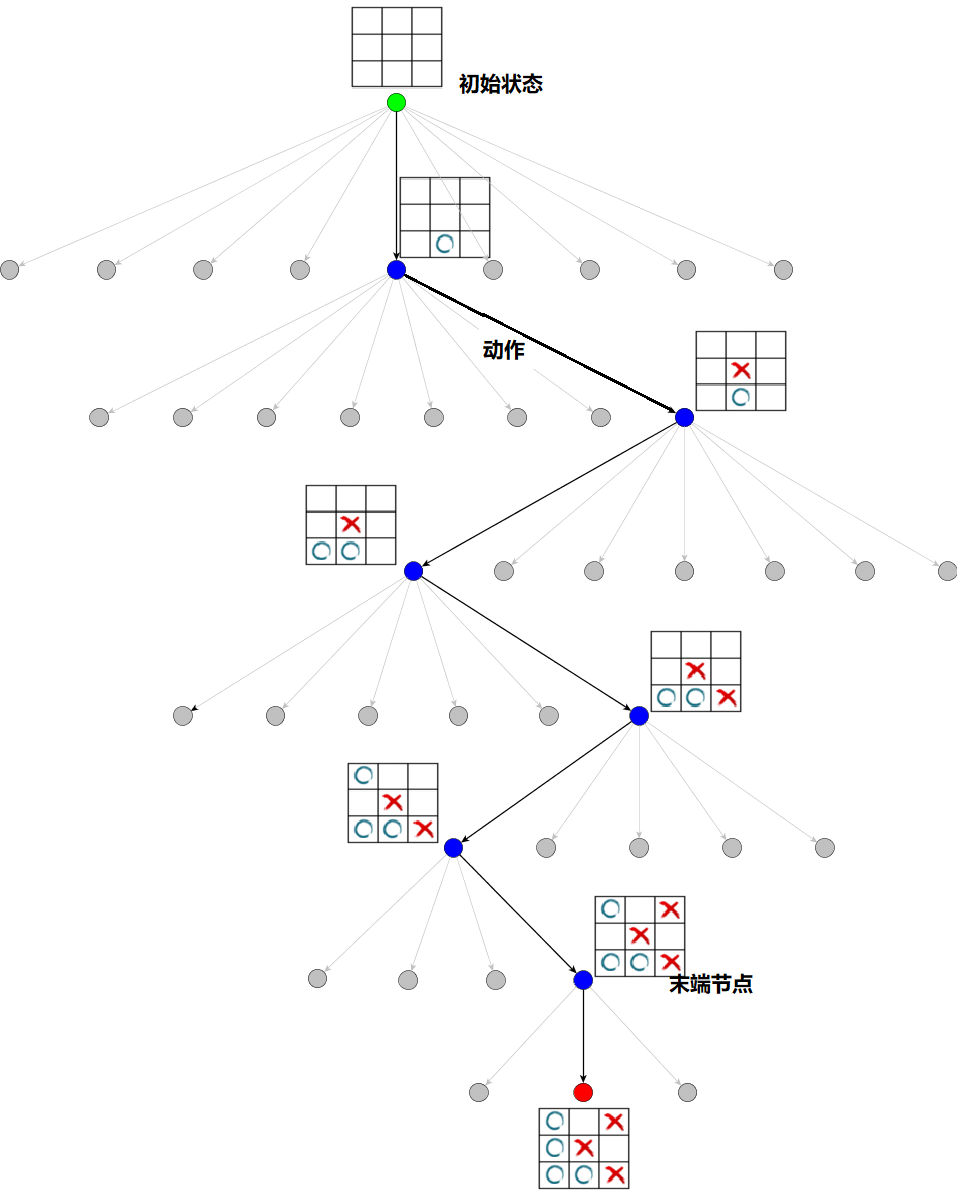
\includegraphics[width=\hsize]{example/tree.png}
	\bicaption[这里将出现在插图索引]
	{博弈树示意图}
	{The Diagrammatic Drawing of Minmax Search Tree}
	\label{tree}
\end{figure}

在博弈树中根节点代表了起始状态信息,从一个节点到其子节点的过程称为动作,节点的子节点数称为分支因子,博弈树的末端节点是博弈无法继续进行的节点,携带了游戏结束的奖励信息。博弈树是一种递归的数据结构,在每次进行一次行动后,根节点的子节点又作为下一状态信息的根节点进行进一步搜索工作。对于选择动作的方案最简单的想法就是建立一颗极小极大搜索树,其示意图如下:

\begin{figure}[!htp]
	\centering
	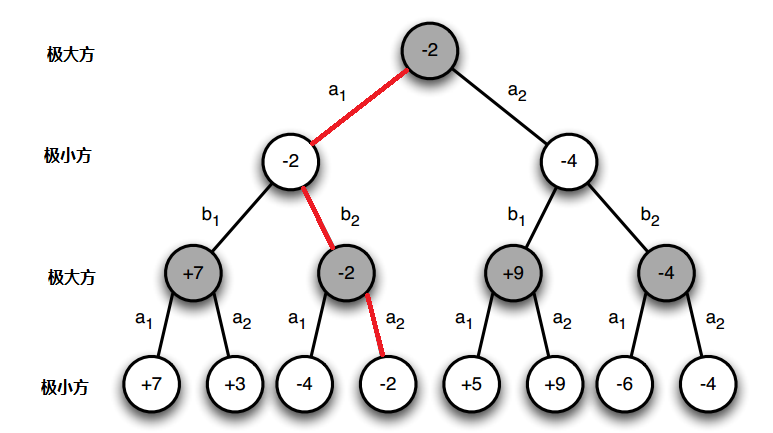
\includegraphics[width=\hsize]{example/minmax.png}
	\bicaption[这里将出现在插图索引]
	{极小极大搜索树}
	{The Diagrammatic Drawing of Minmax Search Tree}
	\label{极小极大搜索树}
\end{figure}
极小极大树提出的核心是在损失尽量小的前提下增加本方的收益,对于示意图来说,在第一步黑方是极大方,在动作选择的过程中会选择尽可能大的收益-2,对于白方来说是极小方,在第二层动作选择时会选择第二层为-2 的子节点-2,图中红色的线代表当前状态的搜索路径。这样一直循环进行选择知道游戏结束,就可以知道当前棋局下所有动作的好坏,越接近最后一步奖励的动作越被鼓励选择。但是对于搜索空间比较大的情况,遍历所有的可能是不现实的,这就需要建立更加高效的搜索树。考虑到深度网络有强大的拟合能力,可以用神经网络拟合最后的输出结果代替真实结果$v(s,w) \approx {v_*}(s)$,这样能提高搜索树的效率。此外由于会存在大量低质量的子树分支,如何在优良分支进行更多扩展,砍掉不需要的子树分支也是另一个难点。
为了解决搜索树过于庞大的问题,蒙特卡洛树应运而生,蒙特卡洛树的思想是从当前给定状态开始,随机采样后续棋局模拟,得到模拟结果,经过多次随机采样将结果的平均值返回该节点作为评估成功率的信息。一般来说节点的数据结构包括以下三个部分${Q,N,W}$,其中$Q(v)$ 为经过该节点s所获得的总评分,N为该节点及其子节点被访问的次数,W为总的奖励收益。
一个完整的蒙特卡洛树包括四个步骤如图\ref{fig:treesearch}:

\begin{figure}[!htp]
	\centering
	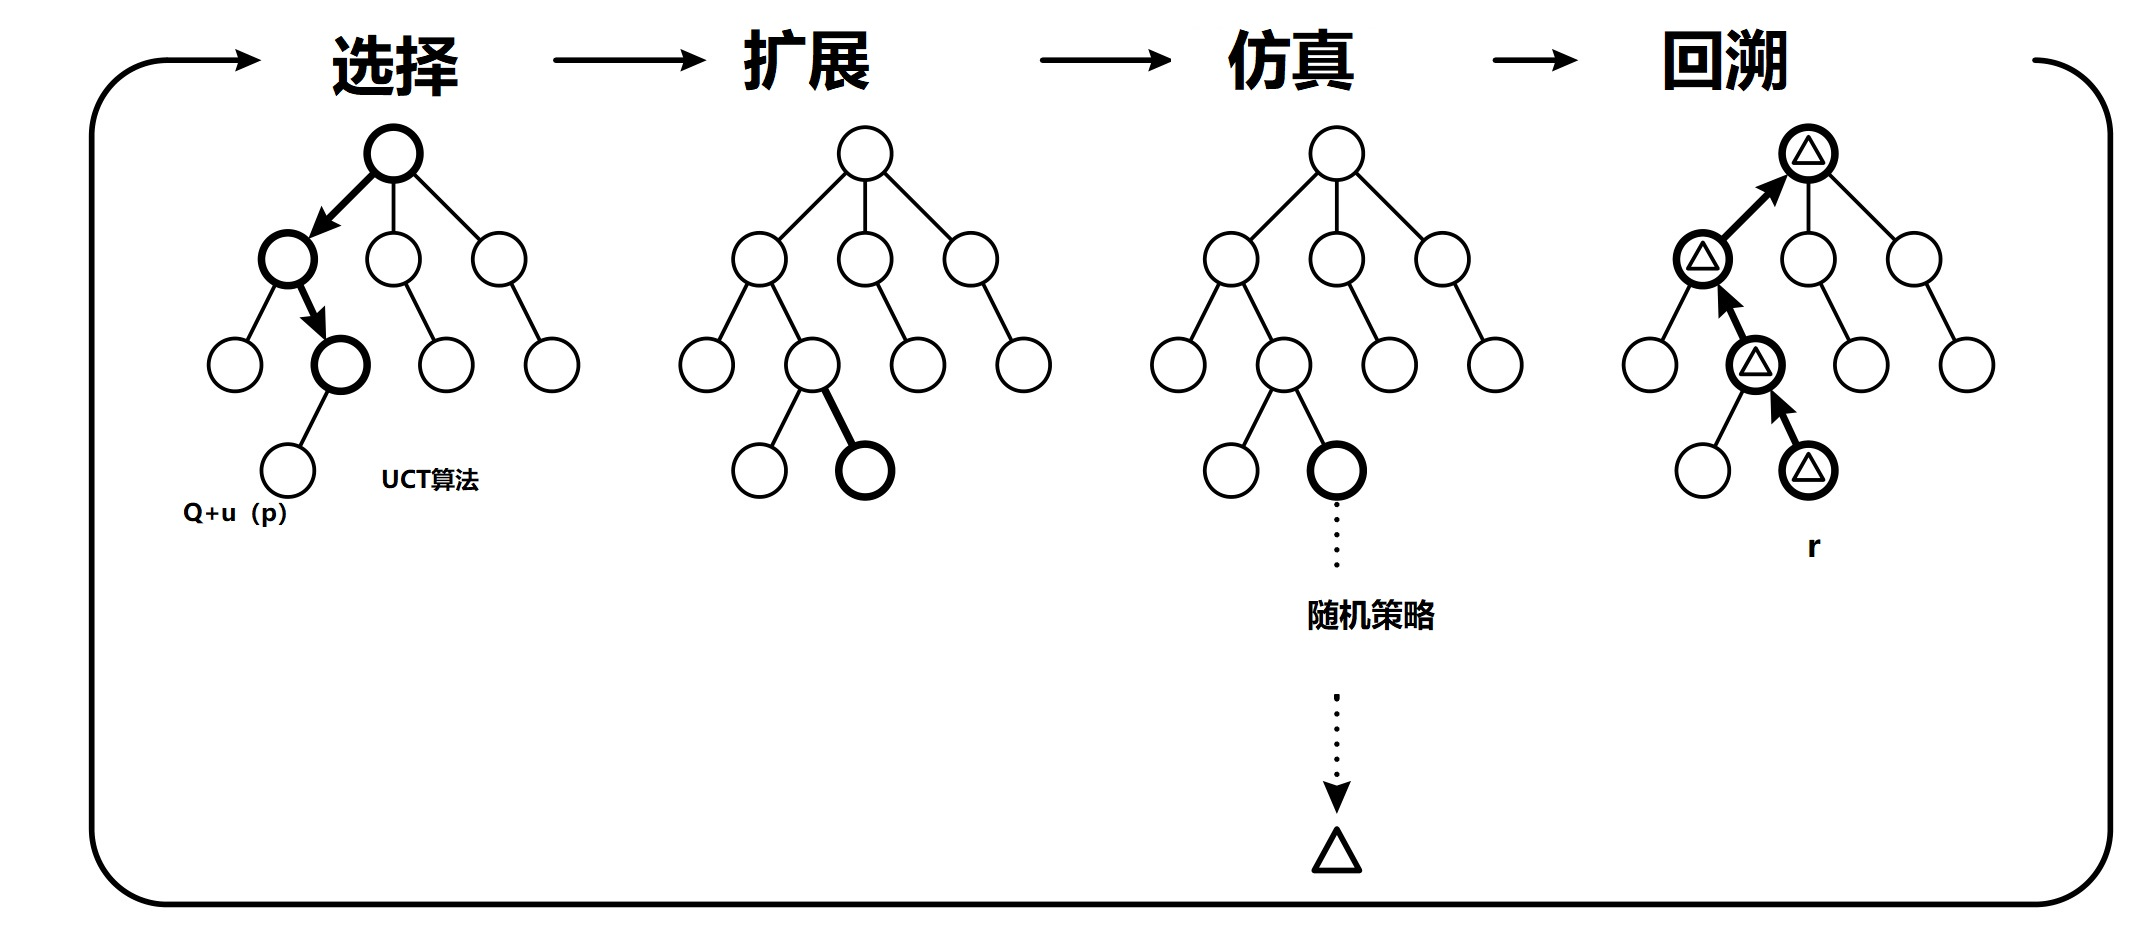
\includegraphics[width=\hsize]{example/treesearch.jpg}
	\bicaption[这里将出现在插图索引]
	{搜索树搜索示意图}
	{The Diagrammatic Drawing of Minmax Search Tree}
	\label{搜索树搜索示意图}
\end{figure}
\begin{enumerate}
	\item 选择(Selection):对于已经建立好的搜索树从根节点向下扩展到子节点选择路径的方案。
	\item 扩展(Expansion):对于没有建立好的树节点部分,在抵达叶节点其分支结构不是终止的叶子节点,在这个叶节点下建立新的叶节点。
	\item 模拟(Simulation):在上一步新建立的叶节点开始,为了评估其选择动作的好坏,随机的进行一系列动作直到结束,建立结果${\rm{R = }}\left\{ {\begin{array}{*{20}{c}}
		{{\rm{1,win}}}\\
		{{\rm{ - 1,loss}}}
		\end{array}} \right.$
	\item 回溯(Backpropagation):利用最终奖励值,把结果返回给从$C$到根节点的连边信息:$Q \leftarrow \frac{W}{N},W \leftarrow W + R,N \leftarrow N + 1$
\end{enumerate}

下面分别介绍这几个步骤的具体实现过程

在选择过程,通常利用到UCT函数,UCT算法相对于传统真正随机的模拟过程减少了前期大量的尝试探索过程,通过迭代的构建子树,能够在每一步进行选择的时候考虑到之前所获取的先验函数信息。
在蒙特卡罗树搜索树遍历过程中,要遵循节点UCT最大化。UCT函数的定义为:
\begin{equation}
UCT({v_i},v) = \frac{{Q({v_i})}}{{N({v_i})}} + c\sqrt {\frac{{\log (N(v))}}{{N(vi)}}} 
\end{equation}

在这里$v$代表当前节点,$ v_i$ 代表其子节点,UCT算法一定程度解决了强化学习算法中最大的问题,即探索和利用的平衡问题。公式的左边是利用部分(exploitation component),用总模拟奖励除以总访问次数可以被理解为一个赢/输的比率,右边的探索部分(exploration component)有效的避免了动作选择陷入局部最优解,让树能够有效的遍历更多未被访问或者访问次数很少的节点,为其提高更大的概率。简单来说就是一个节点的信息由奖励和访问次数构成,具有较高平均奖励的节点值得访问,具有较低访问次数的节点也鼓励被开发。这里$c$是控制探索和利用平衡关系的参数。
扩展过程中由rollout选中的策略并不认为是已展开的节点,只有当搜索到达当前节点,并真实进行动作才认为当前节点被展开。
在模拟过程:为了得到最后的得分结果,当访问到之前没有访问过的节点时,需要进行模拟过程得到预计的奖励,也就是rollout函数。模拟相当于是一个随机过程,通常用服从均匀分布的随机采样得到。在这里rollout是根据专家数据利用浅层网络训练出来的。
这样一个完整的蒙特卡洛搜索过程就得到了,但是由于搜索空间很大,使得搜索速率会下降,Alphago 结合了深度学习模型和强化学习模型完善了蒙特卡洛搜索树的搜索过程。

\subsection{AlphaGo算法原理}
AlphaGo成功的把监督学习网络和强化学习原理结合在一起,其主要思路是利用专家数据作为先验知识指导强化学习算法中的动作选择和评估方案。具体体现在蒙特卡洛搜索树搜索方式中。
AlphaGo由两种网络共四个神经网络系统组成:利用专家数据的监督学习网络和用自我博弈方式产生数据的强化学习网络。如图\ref{fig:net}所示。

\begin{figure}[!htp]
	\centering
	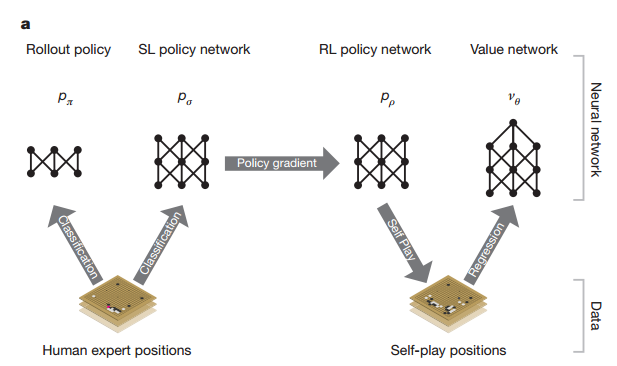
\includegraphics[width=\hsize]{example/net.png}
	\bicaption[这里将出现在插图索引]
	{深度学习网络组成}
	{Neural network training pipeline}
	\label{fig:net}
\end{figure}
首先利用人类专家数据进行训练如下两个网络:基于快速走子策略的${\rho _\pi }$网络,这是一个浅层的快速网络用来给蒙特卡洛搜索树的模拟阶段提供评估信息,相当于是一个多分类的问题。其输入是当前局面信息,输出是各个位置的落子概率。基于监督学习的深层网络${\rho _\sigma }$,相对于rollout policy网络这个网络更加深层,拟合能力更强,相对速度更慢,这个网络是为后面前后学习策略网络初始化参数信息,同时为蒙特卡洛搜索树中在动作选择时提供先验的动作概率。
接着基于强化学习原理,建立两个网络,一个是基于策略的${\rho _\rho }$网络,和历史经验池中的网络进行相互博弈,最大化自己的奖励输出。一个是基于状态价值的${v_\theta }$网络,这个是基于前面博弈数据利用回归的原理进行建立的。在这里,策略网络和价值网络输入都是原始的棋盘信息,策略网络输出的是每个可以落子位置的概率,概率越大代表当前选手得分越高,这个网络也相当于是一个多分类网络,通过不断和自己经验池中的其他网络进行自我博弈来提升效果。价值网络输出是当前状态的评分,相当于一个回归网络。这两个网络分开进行训练如图\ref{fig:policyandvalue}
\begin{figure}[!htp]
	\centering
	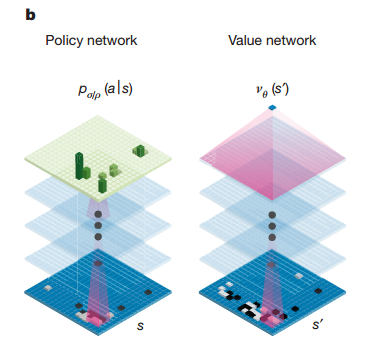
\includegraphics[width=10cm]{example/policyandvalue.png}
	\bicaption[这里将出现在插图索引]
	{策略网络和价值网络结构}
	{Neural network training pipeline}
	\label{fig:policyandvalue}
\end{figure}
\subsection{AlphaZero算法原理}
AlphaZero的出现巅峰了传统机器学习依赖大量数据的需求。根据白板理论,用专家数据学习到的结果并不一定都是可靠的,因此AlphaZero认为数据的产生不一定需要依赖人类专家数据,事实证明,这个理论效果好的超出预期:在只有8个小时的训练时间里击败了AlphaGo,又在4个小时的训练后击败了顶级国际象棋引擎Stockfish,又经过2个小时的训练后击败了日本Elmo引擎。不利用人类数据却得到了比专家方案更好的解决方案,人工智能又上了一大步。
Alphazero 相比于AlphaGo做了如下改进:
\begin{enumerate}
	\item 首先在特征的提取上面,Alphazero不再使用经过人工处理的特征,而选择原始的棋盘信心作为系统的输入,真正实现了端到端。特征提取工作直接由深度学习网络进行。
	\item 在蒙特卡洛树快速走子策略的时候,不再使用随机走子,或者利用专家数据训练快速走子策略,而直接使用强化学习策略梯度网络进行快速走子。这样提高了蒙特卡洛树预估结果的准确性。
	\item 在网络结构层面,简化了网络形式,由于不再使用监督数据,和快速走子网络,主体网络只有策略网络和价值网络。这两个网络前期特征提取工作大同小异,所以对网络进行了合并操作,大大降低了网络的复杂度。这样以轻微增加策略网络的预测错误率为代价大大降低了价值网络预测的误差。
\end{enumerate}

。Alphazero对UCTS进行了改进,每次动作选择最大化上限置信区间:
\begin{equation}
{\rm{Q(}}\mathop s\limits^ \to  {\rm{,}}\mathop a\limits^ \to  {\rm{) + U(}}\mathop s\limits^ \to  {\rm{,}}\mathop a\limits^ \to  {\rm{)}}
\end{equation}
其中,${\rm{U(}}\mathop s\limits^ \to  {\rm{,}}\mathop a\limits^ \to  {\rm{)}} \propto \frac{{P(\mathop s\limits^ \to  ,\mathop a\limits^ \to  )}}{{1 + N(\mathop s\limits^ \to  ,\mathop a\limits^ \to  )}}$。Q是定义的叶子节点的值,将会在下面提到。

叶子节点扩展的方式也不再是基于监督学习网络得到的先验概率,而是依据强化学习网络端策略网络输出的策略概率。每个叶子节点存储了以下信息:先验概率$P(\mathop s\limits^ \to  ,\mathop a\limits^ \to  )$,访问次数$N(\mathop s\limits^ \to  ,\mathop a\limits^ \to  )$,行动价值$Q(\mathop s\limits^ \to  ,\mathop a\limits^ \to  )$。
在模拟过程,每遍历一条边更新统计数据,访问次数${N(\mathop s\limits^ \to  ,\mathop a\limits^ \to  )} +=1$,更新行动价值:$Q(\vec{s},\vec{a})=\frac{1}{N(\vec{s},\vec{a})}\sum_{\vec{s}'\vert \vec{s},\vec{a}\Rightarrow \vec{s}'}V(\vec{s}')$, 其中$\vec{s}'\vert \vec{s},\vec{a} \Rightarrow \vec{s}'$表示模拟过程中从$\vec{s}$走到$\vec{s}'$的所有落子行动$\vec{a}$。
在回溯的阶段,
根据UCT算法向下遍历叶子节点,直到得到最后的结果,进行回溯操作。
在网络结构上,使用一分为二的形式,即前期特征提取部分使用相同的网络结构,因为策略网络输出的是多分类问题,所以最后一层用全连接加softmax函数,损失函数为交叉熵。而价值网络是回归问题,最后一层用sigmoid函数,损失函数为均方误差损失函数。拟合的数据就是前期蒙特卡洛搜索树搜索得到的结果。
把蒙特卡洛树和深度学习网络组合在一起的示意图如下\ref{fig:Alphazero1}:

\begin{figure}[!htp]
	\centering
	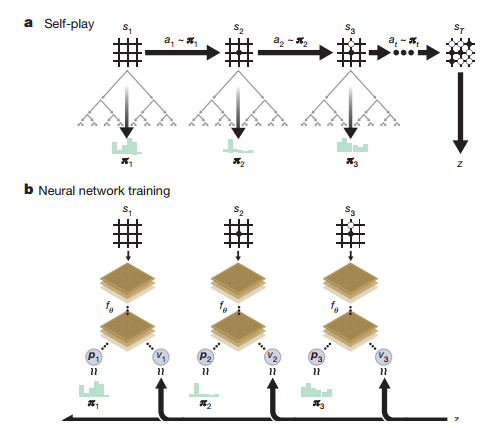
\includegraphics[width=10cm]{example/Alphazero1.png}
	\bicaption[这里将出现在插图索引]
	{AlphaZero 模型示意图}
	{Neural network training pipeline}
	\label{fig:Alphazero1}
\end{figure}
通过蒙特卡洛树得到每个状态下的$({s_t},{\pi _t},{z_t})$,其中$s_t$表示$t$时刻的状态信息,$\pi_t$表示$t$时刻蒙特卡洛搜索树的动作分布,定义为:
\begin{equation}
\label{eq:fenbu}
{\pi _{\rm{t}}}(a|{s_t}) = \frac{{N({s_{\rm{t}}},a)}}{{\sum\nolimits_b {N({s_t},b)} }}
\end{equation}
最后神经网络拟合的损失函数如下:
\begin{equation}
l = {(z - v)^2} - {\pi ^T}\log p + c{\rm{||}}\theta {\rm{|}}{{\rm{|}}^2}
\end{equation}
其中$v$和$p$分别是策略价值网络输出的评分值和动作概率值。
\section{一种改进的AC强化学习算法}
正如经典算法提到,强化学习面临的主要问题是探索和利用的平衡问题,当探索能力越强,对应的搜索树的宽度越深,利用能力越强,树的深度越深,最后结果可能会陷入局部最优解。在AlphaZero中利用了UCTS算法进行动作的选择,算法主要思想就是指导动作选择的概率。在本章对UCTS动作选择部分进行了改进,引入随机噪声,鼓励动作选择更多没有访问的节点,避免陷入局部最优的可能性。同时在神经网络的拟合部分结合训练结果用到自适应学习率的方法,加快网络前期的训练过程,在越接近最优解时缩小学习率。
算法整体示意图如图\ref{fig:ACgaijin}所示。
\begin{figure}[!htp]
	\centering
	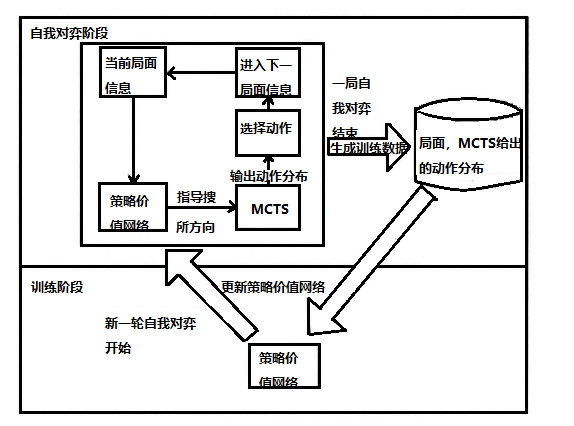
\includegraphics[width=10cm]{example/Alphazero.png}
	\bicaption[这里将出现在插图索引]
	{改进AC算法工作示意图}
	{Neural network training pipeline}
	\label{fig:ACgaijin}
\end{figure}
可见数据流的流向是先由蒙特卡洛树搜索得到相应的动作概率以及得分数据,然后把数据传向深度学习网络。由于自对抗生成式数据生成过程比较缓慢,提高样本利用率,有效平衡探索和利用的关系对于模型的效果有重要的作用。本节提出了两点改进,一是在神经网络学习阶段用自适应学习率的方法适应数据前期不稳定,后期接近标签奖励明确的特点,二是在统计蒙特卡洛搜索树信息中引入温度常数和噪声系数,促进前期探索后期利用的学习过程。
\subsection{基于交叉熵信息的自适应学习率}
在原来的Alphazero论文算法中,学习率的算法是根据迭代次数进行调整,寻求最优解的方式为异步随机梯度下降法,初始化的学习率为$\alpha$,当迭代次数为$T$时递减一半,为$2T$时再次递减,直到寻得最优解,这样学习率$\alpha$以及时间$T$都需要人为进行选取,当参数选取不合适很容易导致梯度不稳定过拟合或欠拟合现象的出现。而且迭代次是并不一定能直接反应出网络梯度更新效果的好坏,调参负担重导致结果容易出现崩溃的现象。这里我们选取能够直接反应网络更新前后变化量大小及效果的距离度量--相对熵作为衡量是否需要调整步长的指标。相对熵的定义如下:
\begin{equation}
{\rm{D}}(P{\rm{||Q}}){\rm{ = }}\sum\limits_{x \in X} {p(x)\log \frac{{P(x)}}{{Q(x)}}} 
\end{equation}

这里根据相对熵的变化自适应调整学习率,由于交叉熵能够直接反映出网络结构对策略拟合能力的好坏,当相对熵变化大于一定阈值后,说明更新前后的网络有了较大的改变,通常我们希望网络能够缓慢逐步向需要更新的方向进行改变,这时候可以适当减小学习率,反之,当交叉熵变化小于一定的阈值说明网络更新梯度过于平稳,为了提高收敛速度,可以适当加大学习步长。结合强化学习网络,定义前后差距为:
\begin{equation}
\label{eq:dist}
dist =  - \sum\limits_{i = 1}^{|A|} {{p_{\bar \theta }}(s)(\log ({p_\theta }(s)) - \log ({p_{\bar \theta }}(s))} )
\end{equation}

这里,$p_{\bar \theta}$代表状态更新前的网络参数,$p_\theta $代表状态更新后的网络参数,式\ref{eq:dist}代表了网络更新前后的变化程度相对于原来网络的变化程度。因此可以根据这个变化程度自适应调整学习率:
\begin{equation}
\label{eq:r}
r = \left\{ {\begin{array}{*{20}{c}}
	{r/\lambda ,dist > threshold\_up}\\
	{r,others}\\
	{r*\lambda ,dist < threshold\_down}
	\end{array}} \right.
\end{equation}
其中,$\lambda$代表每次更新学习率放缩的比例,$threshold\_up$和$threshold\_down$分别代表了上限阈值和下限阈值。
\subsection{引导式对弈探索}
为了进一步解决强化学习探索和利用的平衡问题,式\ref{eq:fenbu}已经介绍了经过蒙特卡洛搜索树搜索后统计的状态动作概率值,考虑到动作选择的概率很大程度依靠于蒙特卡洛树多次模拟得到的统计结果,在网络训练初期,很多时候蒙特卡洛的动作选择是随机性的,对神经网络的拟合借鉴性不大,而在网络后期,越接近奖励的步骤目标越明确,这时候可以增大对应的借鉴比例。这里引入温度常量$\tau $,动作概率公式变为:
\begin{equation}
\label{eq:gailu}
{\pi _t}(a|{s_t}) = \frac{{{e^{N{{({s_t},a)}^{1/\tau }}}}}}{{{e^{\sum\nolimits_b {N{{({s_t},b)}^{^{1/\tau }}}} }}}}
\end{equation}
在这里${N({s_t},a)}$是在状态$s_t$时选择动作$a$的次数,${\sum\nolimits_b {N{{({s_t},b)}^{1/\tau }}} }$是在状态$s_t$时,选择所有动作的总次数,这里面温度常数$\tau>0$,是控制探索和利用平衡的指标,$\tau$越小,代表动作策略更倾向于选择访问次数多的动作,当$\tau$趋近于零时函数趋近于仅利用,$\tau$越大,动作概率趋近于选择更多未探索到的策略,$\tau$趋近于正无穷,策略趋近于仅探索。这里可以在开局把$\tau$设为一个较大的初值,鼓励智能体探索不同情况的动作,在训练的后期,令$\tau  \to 0$,当训练策略稳定后,智能体将选择访问次数较多的动作。
这里为了进一步增加探索的几率,对动作概率引入随机噪声:
\begin{equation}
\label{eq:zaosheng}
	P({s_t},a) = (1 - \varepsilon ){\pi _t}(a|{s_t}) + \varepsilon {\eta _a}
\end{equation}
其中,${\pi _t}(a|{s_t})$即为\ref{eq:gailu}中的动作概率值。${\eta _a} \sim {\rm{Dir}}(c)$中$c$为狄利克雷噪声(Dirichlet noise)中的常数,$\varepsilon$为平衡噪声和概率值的常数。
所以改进后的自适应学习率调整的算法流程如下:
\begin{algorithm}[!htpb]
	\caption{基于相对熵的自适应学习率强化学习算法}% Ëã·¨±êÌâ
	\begin{algorithmic}[1]
		\Require ~~ \\
		初始学习率$r_0$,上限阈值$threshold\_up$和下限阈值$threshold\_down$,调整率$\lambda$,网络初始参数$\theta_0$,以及温度常数$\tau$和狄利克雷常数$c$,平衡系数$\varepsilon $。
		\While {没有达到网络优化停止准则}
		\State 从经验池中采样m个样本${\rm{\{ }}{{\rm{x}}^{(1)}}{\rm{,}}{{\rm{x}}^{(2)}}{\rm{,}}...{\rm{,}}{{\rm{x}}^{(m)}}{\rm{\} }}$
		\State 根据式\ref{eq:gailu}统计在$t$时刻状态$s_t$下选择不同动作的概率。
		\State 根据\ref{eq:zaosheng}更新概率值。
		\State 当利用神经网络进行概率值拟合时,根据式\ref{eq:dist}计算网络参数更新前后相对变化量。
		\State 然后利用式\ref{eq:r}更新学习率。进行下一轮蒙特卡洛树的更新和神经网络参数的更新
		\EndWhile
	\end{algorithmic}
\end{algorithm}
\section{针对五子棋双人博弈场景进行模型性能分析}
在本章,主要针对上一节提出的两点改进算法进行模型参数性能的分析,根据分析曲线和具体的应用场景进行参数的选择。由于研究的是博弈式游戏策略,因此以五子棋为实验背景进行多组对比实验。

\subsection{数据及场景介绍}
五子棋是大家耳熟能详的简单棋类游戏,其游戏规则比较简单,在一个$n\cdot n$的棋盘里,黑手和白手交替进行一次落子,可落子的空间为全盘,所以在搜索树的每一层节点都有n*n种可能性。当玩家首先在棋盘中在横向纵向以及对角上连成连续的五个棋子即判定为获胜。
抽象成强化学习模型,为了表示黑白双方的位置信息,这里用4层的8*8的棋盘表示落子信息。第一层为当前玩家全部落子位置,有子的位置为1,没有子的位置为0,同样的,第二层表示对方玩家全部落子位置,第三层为对手最后一步落子的位置,在这一层特征中只有一个位置为1,剩下位置都为0。由于是极小极大化的过程所欲需要最后一层平面表示当前玩家是黑方还是白方,黑方为全1的矩阵,白方为全0的矩阵。在动作方式的建立上,由于棋盘可落子范围为全盘,所以初始化动作为8*8的概率矩阵,当某一位置以落子,将该位置从动作池中抽掉。由于五子棋是有严格胜负规则的游戏,所以奖励可以根据游戏的胜负规则来确定:如果进行到游戏的最后如果当前玩家获胜,奖励为+1,对手奖励为-1,反之如果当前玩家失败,奖励为-1,对手为+1,如果棋盘全满,双方无子可落,双方平局,奖励全部为0。
在利用深度学习网络进行前期特征提取时,所有实验都用4层卷积网络进行特征的提取工作,在输出中,策略网络看成多分类问题激活函数选用softmax函数,价值网络看成回归问题,输出函数用tanh函数。
每下一步用400次蒙特卡洛仿真,经过self-play形式进行博弈数据的生成,把数据放进经验池中,由于五子棋棋盘信息是严格对称的,而博弈数据的产生又是比较缓慢的,所以这里采用对期棋盘数据分别进行90度,180度,270度的翻转操作,这样有效进行了数据扩充,弥补了随机采样带来的样本利用率低的缺点。
\subsection{参数对模型效果影响曲线}
在这一节对比了不同温度参数,不同噪声系数对实验结果的影响。可以通过计算策略网络的信息熵反应策略网络决策的分布离散程度,当信息熵越小,代表策略越明确,当信息熵越大,代表决策过程越趋向于随机。同时监控了神经网络的损失函数随迭代次数变化曲前,当损失函数呈下降趋势说明网络是趋近于收敛的,下降的越平滑说明网络越稳定。
首先对比不同$r$值对各种参数的影响,如图所示:
%\begin{figure}[!htp]
%	\centering
%	\begin{subfigure}{2.5cm}
%		\centering
%		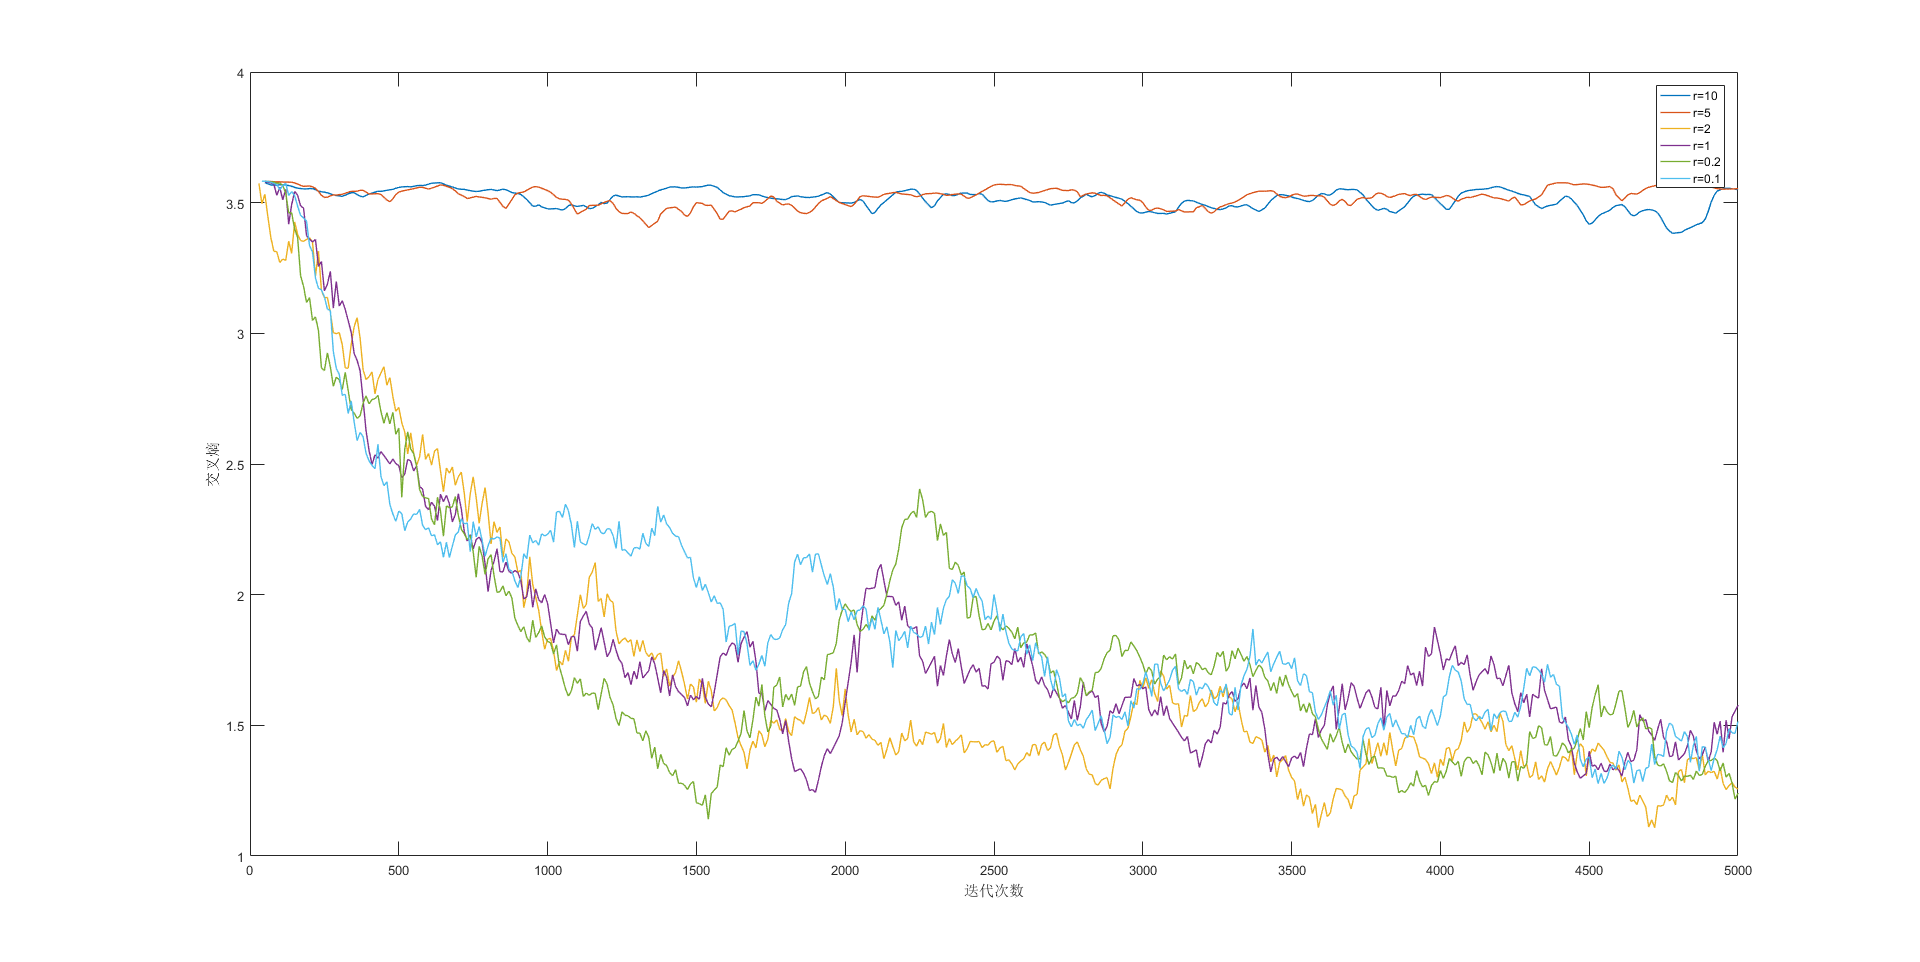
\includegraphics[height=5cm]{example/r-entropy.png}
%		\caption{学习率对交叉熵的影响}{}
%	\end{subfigure}
%	\hspace{4em}
%	\begin{subfigure}{2.5cm}
%		\centering
%		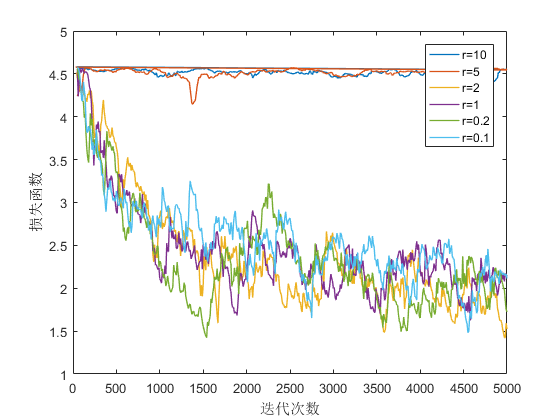
\includegraphics[height=5cm]{example/r-loss.png}
%		\caption{学习率对损失函数的影响}{}
%	\end{subfigure}
% 	\hspace{4em}
% 	
% 	\begin{subfigure}{2.5cm}
% 		\centering
% 		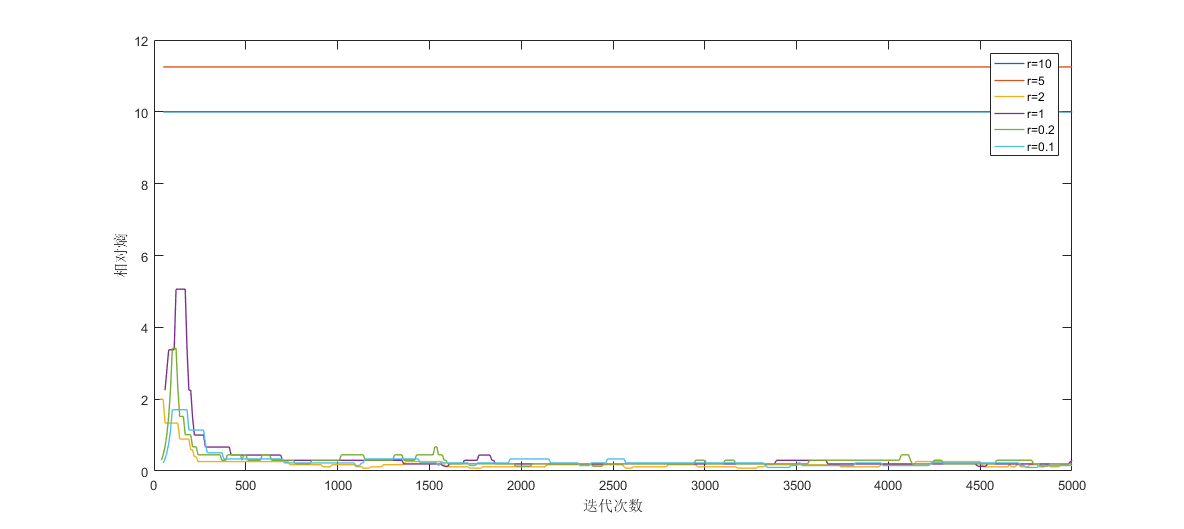
\includegraphics[height=5cm]{example/r-kl.png}
% 		\caption{学习率对相对熵的影响}{}
% 	\end{subfigure}
% 	\begin{subfigure}{2.5cm}
% 		\centering
% 		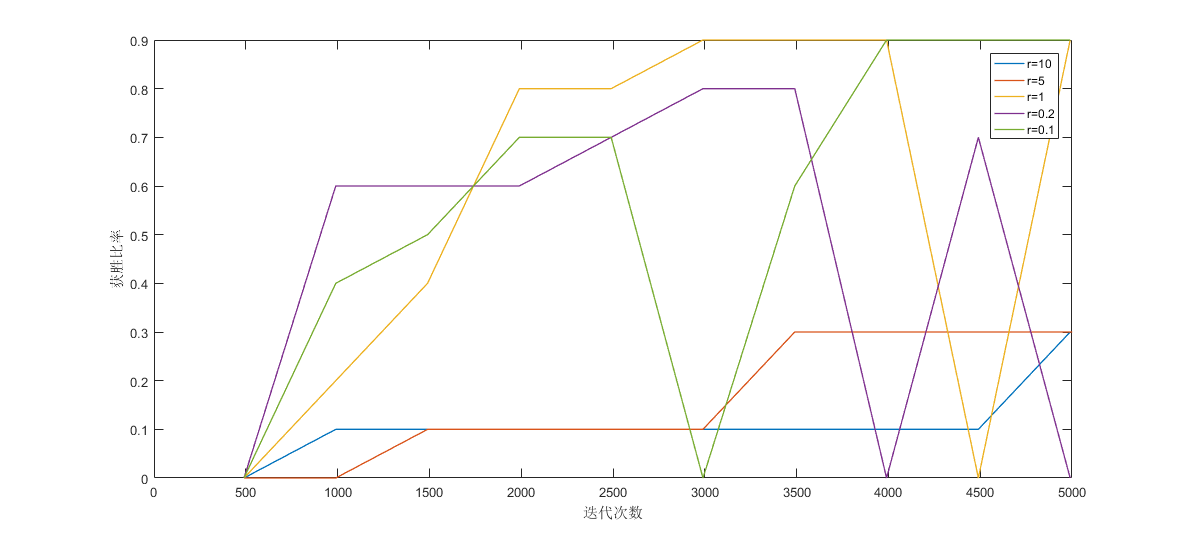
\includegraphics[height=5cm]{example/r-winratio.png}
% 		\caption{学习率对获胜率的影响}{}
% 	\end{subfigure}
%	\bicaption{学习率对不同参数的影响}{}
%	\label{fig:r}
%\end{figure}
%


\begin{figure}[t]
	\centering
	\subcaptionbox{学习率对交叉熵的影响\label{fig1:response:a}}
	{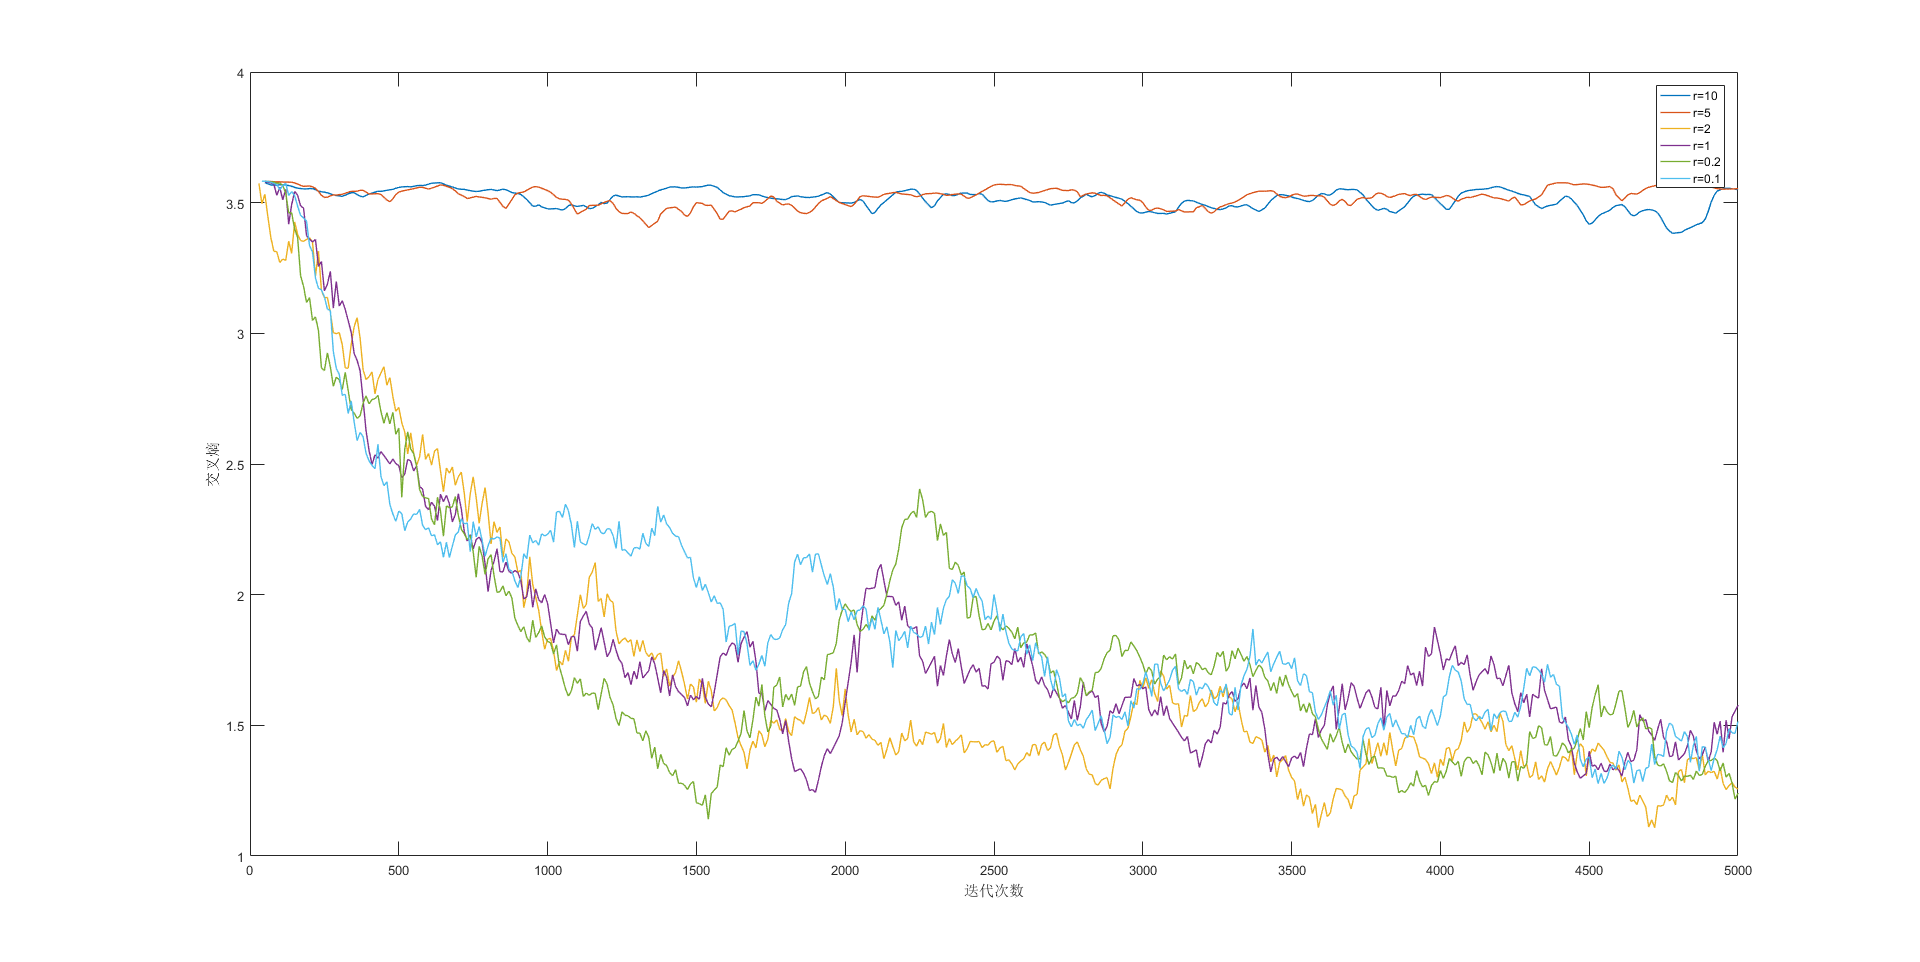
\includegraphics[width=0.45\hsize,height=0.45\hsize]{example/r-entropy.png}}
	\hspace{0.5em}
	\subcaptionbox{学习率对损失函数的影响\label{fig1:response:b}}
	{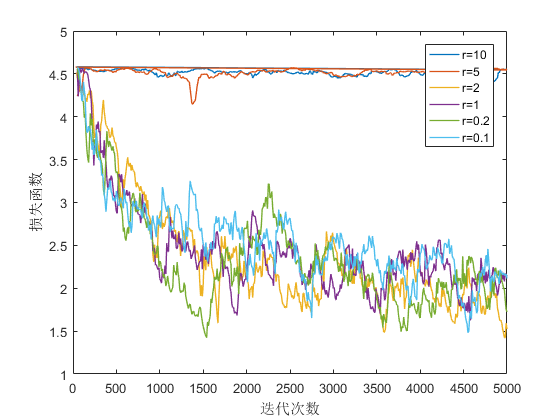
\includegraphics[width=0.45\hsize,height=0.45\hsize]{example/r-loss.png}}
	\newline
	\centering
	\subcaptionbox{学习率对相对熵的影响\label{fig1:response:c}}
	{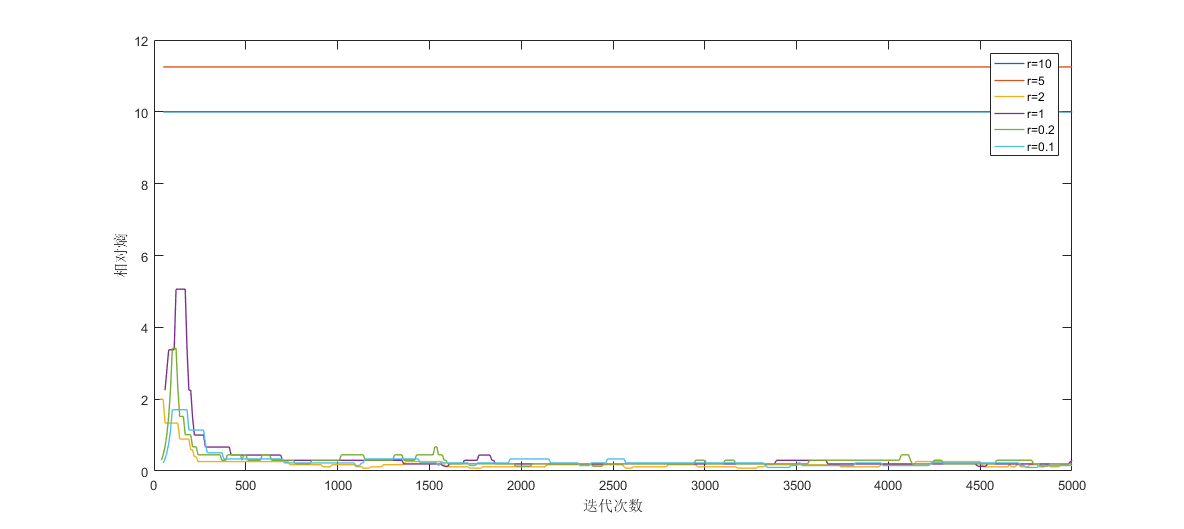
\includegraphics[width=0.45\hsize,height=0.45\hsize]{example/r-kl.png}}
	\hspace{0.5em}
	\subcaptionbox{学习率对获胜率的影响\label{fig1:response:d}}
	{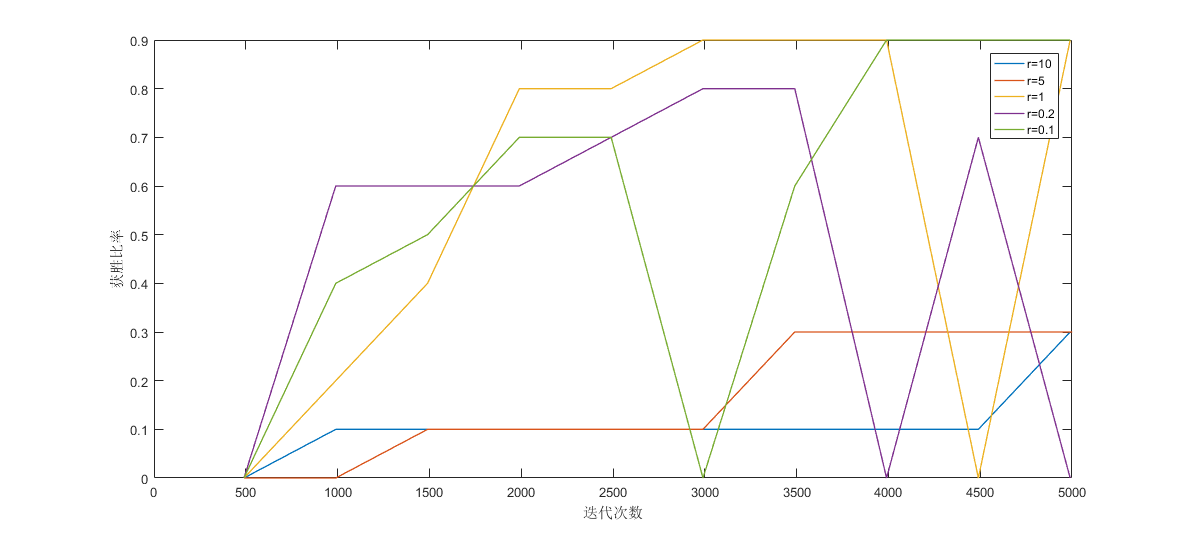
\includegraphics[width=0.45\hsize,height=0.45\hsize]{example/r-winratio.png}}
	\bicaption
	{学习率对不同参数的影响}
	{Examples of response maps during occlusions and not.The first row shows the original and response maps with no occlusions while the second row shows the maps with occlusions. The first column are the shots of sequence bear front in Princeton dataset. The color response maps are in the second column while the depth’s are in the third.}
	\label{fig1:response}
\end{figure}
图\ref{fig1:response:a}展示了不同学习率下策略网络的交叉熵,代表了策略的离散程度。图\ref{fig1:response:b}展示了损失函数随迭代次数的改变,损失函数包括策略网络损失函数和价值网络损失函数,损失函数越小代表网络拟合self-play数据效果越好。图\ref{fig1:response:c}代表了网络参数的相对变化情况,自适应调整学习率时,根据相对熵调整学习率移动方向,所以相对熵稳定在一个相对小值利用模型学习。图\ref{fig1:response:d}代表在训练过程中智能体和一个提前训练好的用rollout策略学习的智能体进行博弈的结果,网络每迭代500次进行一次评估,对战10回合统计获胜比率。
一个好的网络应该交叉熵随着迭代的进行呈下降趋势。当$r$过大时,交叉熵基本不变网络相当于随机输出动作,当$r=10$和$r=5$时可以看出智能体在随机输出动作,神经网络的损失函数没有呈下降的趋势,从获胜比例看获胜率相抵很低。固定迭代次数,交叉熵和损失函数随着学习率减小而减小。但并不是$r$越小越好,当$r=0.1$时从获胜比率看智能体模型并不稳定。

\begin{figure}[t]
	\centering
	\subcaptionbox{温度常数对交叉熵的影响\label{fig2:response:a}}
	{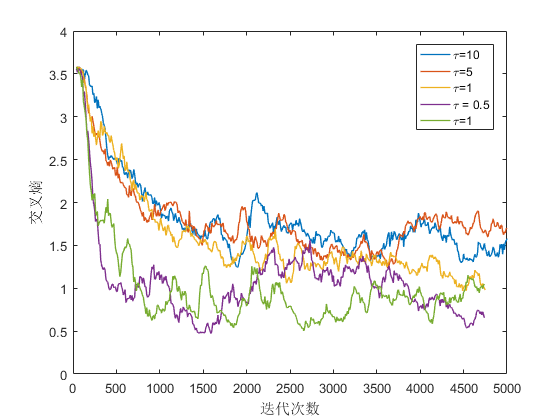
\includegraphics[width=0.45\hsize,height=0.45\hsize]{example/temp-entropy.png}}
	\hspace{0.5em}
	\subcaptionbox{温度常数对损失函数的影响\label{fig2:response:b}}
	{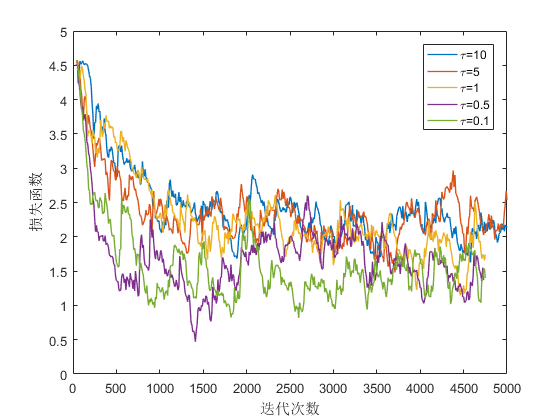
\includegraphics[width=0.45\hsize,height=0.45\hsize]{example/temp-loss.png}}
	\newline
	\centering
	\subcaptionbox{温度常数对相对熵的影响\label{fig2:response:c}}
	{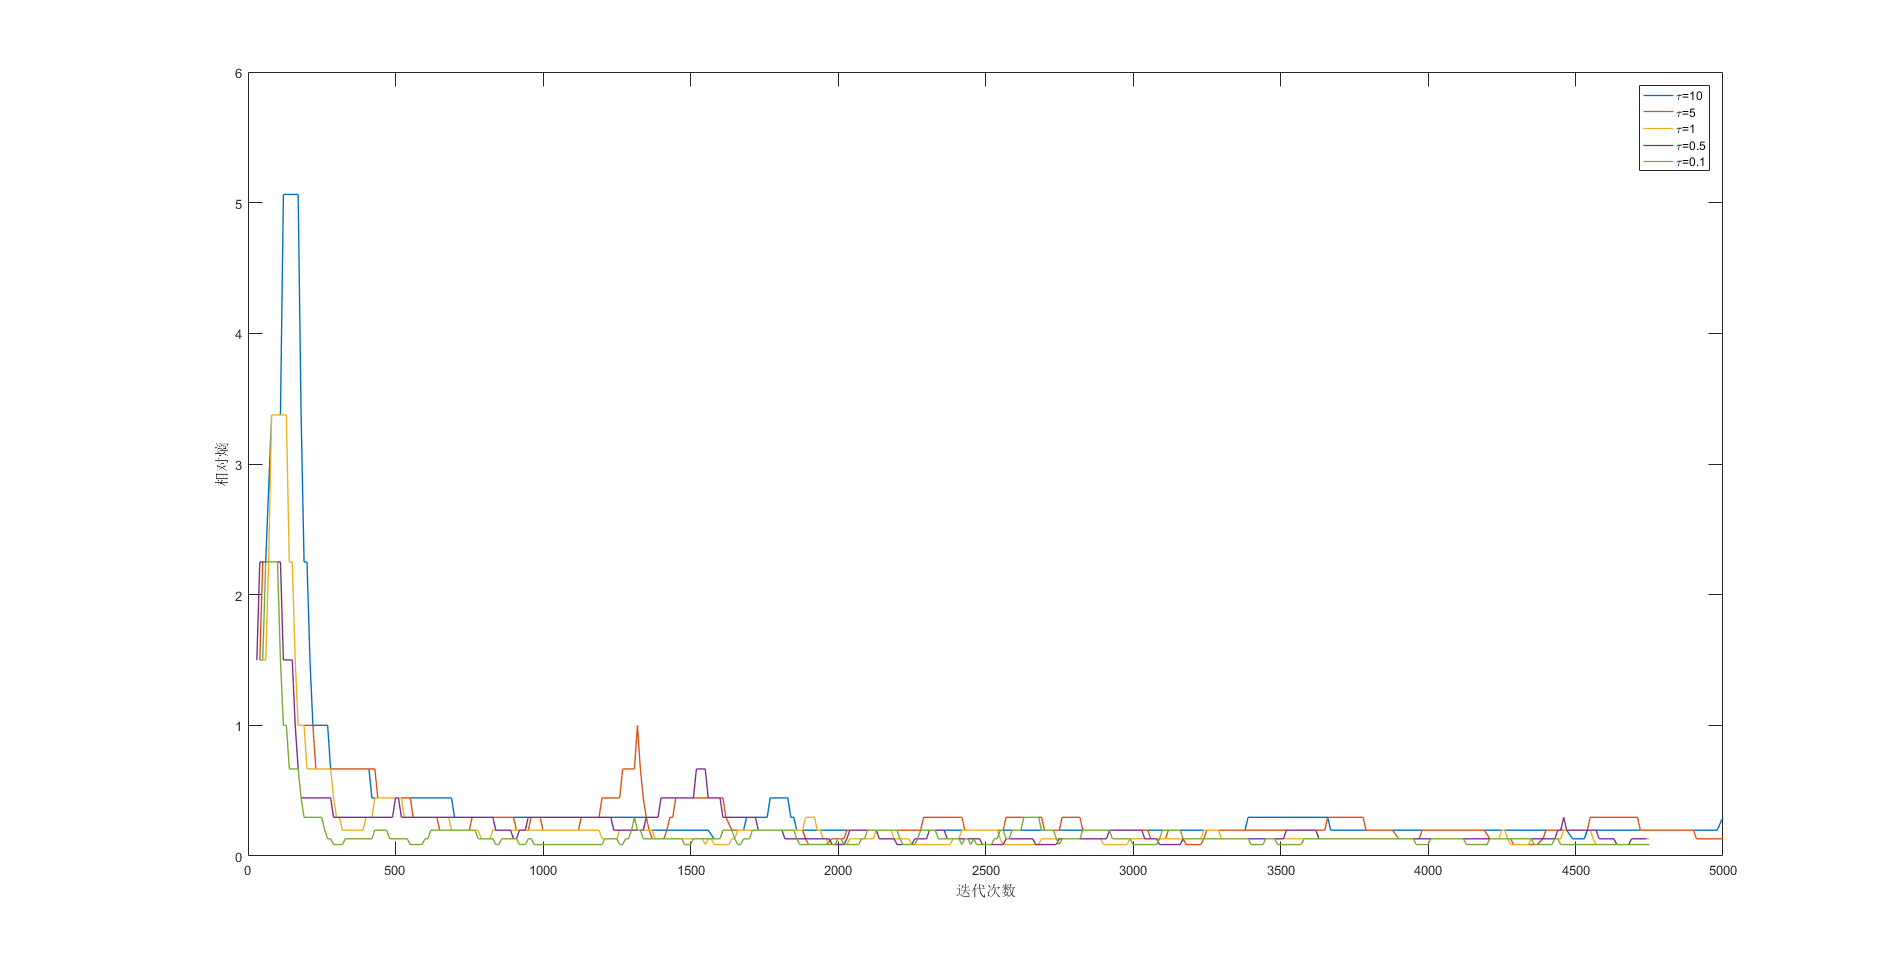
\includegraphics[width=0.45\hsize,height=0.45\hsize]{example/temp-kl.png}}
	\hspace{0.5em}
	\subcaptionbox{温度常数对获胜率的影响\label{fig2:response:d}}
	{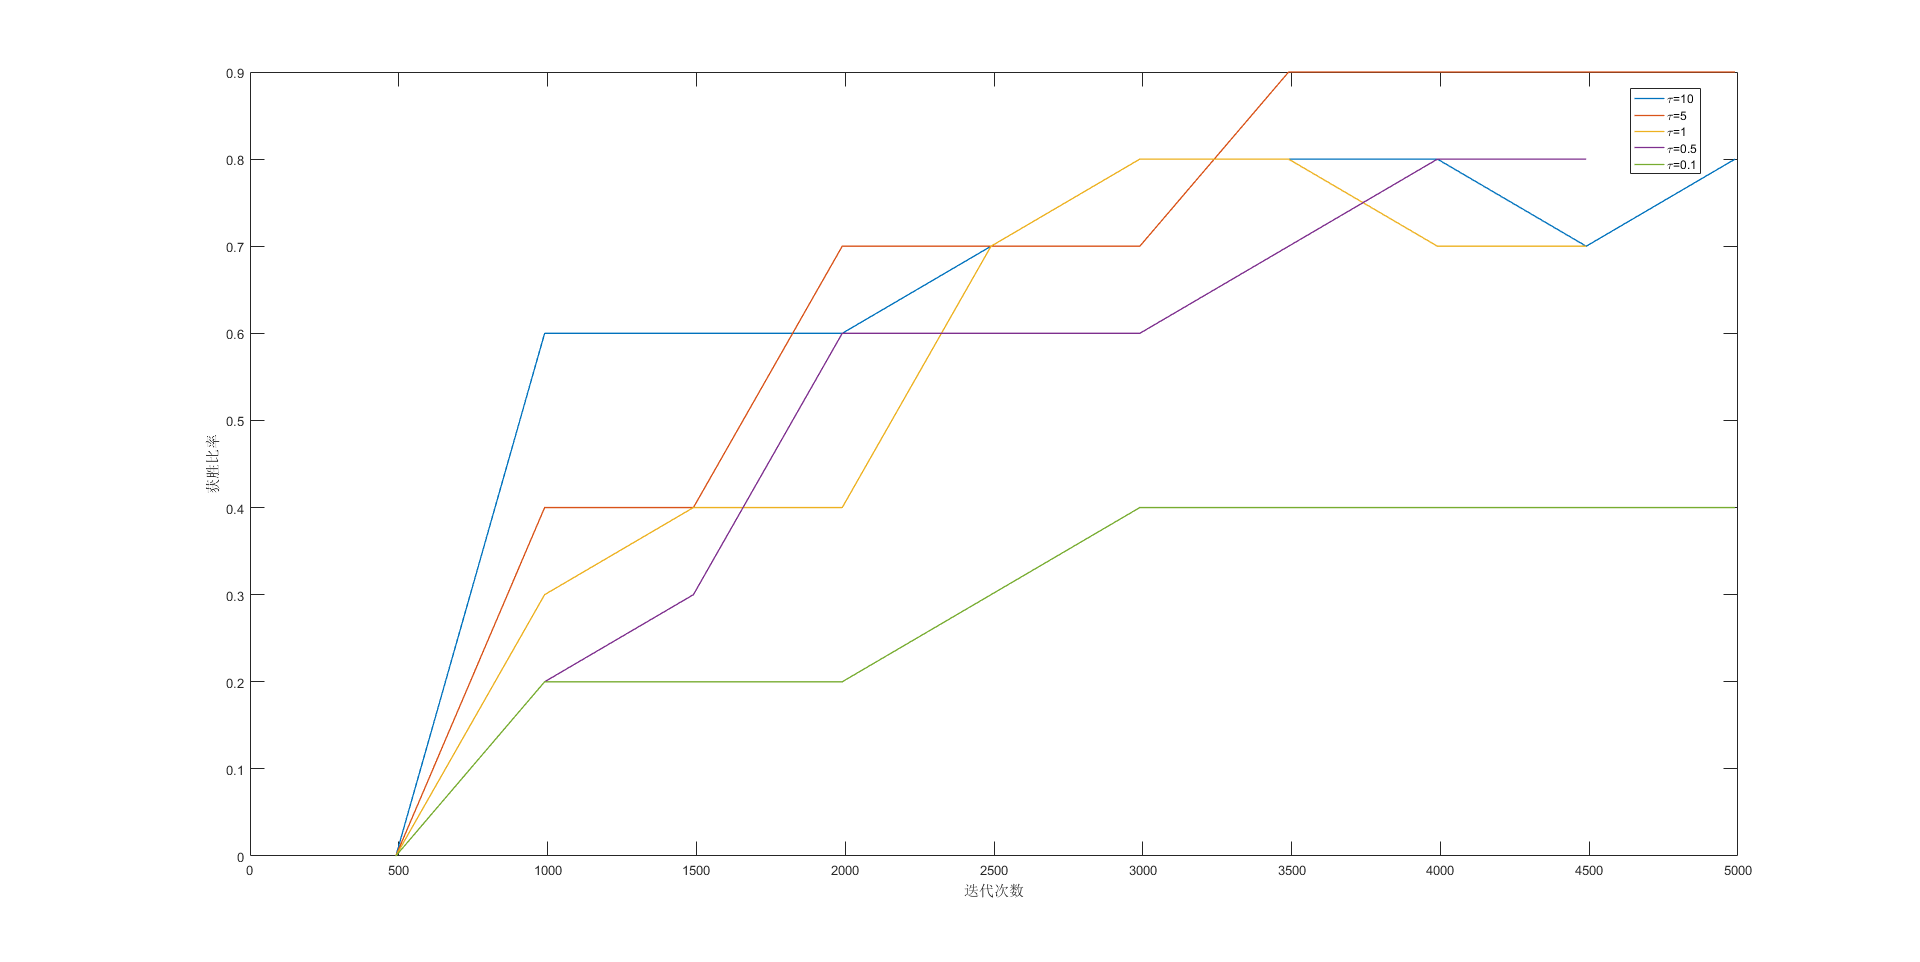
\includegraphics[width=0.45\hsize,height=0.45\hsize]{example/temp-winratio.png}}
	\bicaption
	{温度常数对不同参数的影响}
	{Examples of response maps during occlusions and not.The first row shows the original and response maps with no occlusions while the second row shows the maps with occlusions. The first column are the shots of sequence bear front in Princeton dataset. The color response maps are in the second column while the depth’s are in the third.}
	\label{fig2:response}
\end{figure}
图\ref{fig2:response}展示了温度常数对不同参数的影响,这里面仍以交叉熵,相对熵,损失函数和获胜比率进行对比。
可以看出来,$\tau$越大,策略网络趋向于探索策略,交叉熵下降缓慢,以$\tau=10$为例,从损失函数看,其损失函数下降缓慢,收敛较慢,从获胜率曲线看,其前期表现较其他参数快,因为前期蒙特卡洛搜索得到的结果并不可靠,单纯拟合网络并不是最好的结果,但是由于动作的不稳定性,随着迭代次数增加其获胜率上升比较缓慢。温度系数越小,策略越趋向于仅利用,损失函数下价格呢的会很快,交叉熵也下降的比较快,相当于贪心策略。但是从$\tau=0.1$曲线的获胜率来看,其后期表现很差。所以合理平衡探索和利用对于强化学习问题来说是很重要的。
\section{基于五子棋的单智体博弈实验}

在上一节参数选择经验的基础上,这里我们选取参数信息进行不同算法之间结果比较。本实验对训练过程中神经网络的损失函数信息,学习率,总损失,以及策略端损失和价值网络损失进行对比,证明算法的可行性。策略网络损失代表神经网络动作部分和蒙特卡洛树拟合值的偏差,价值网络代表神经网络和真实值之间回归的偏差,网络优化的总损失函数为策略损失和价值损失之和。这里具体把两个损失函数分开,看不同算法得到的网络模型效果对比。在这里参数信息如下:
\begin{table}
	\centering
	\caption{股票数据回归结果}
	\begin{tabular}{c|c}
		\hline 
		棋盘大小 & 8*8 \\ 
		\hline 
		自适应学习率参数 & 1.0 \\ 
		\hline 
		温度探索参数temp & 1.0 \\ 
		\hline 
		每次落子蒙特卡洛搜索次数 & 400 \\ 
		\hline 
		批训练样本大小 & 500 \\ 
		\hline 
		迭代次数 & 1500 \\ 
		\hline 
	\end{tabular} 
\end{table}


对比不同算法得到的结果:
(加不同算法的曲线图)

最后得到的五子棋模型效果如下:
在初始位置,神经网络对各个位置落子的概率如下:
可以看出,模型倾向于把初始落子位置放在中间,这也符合正常规则的五子棋的下法,第一步越靠近中间越有利。从这个角度说明了网络学习到参数的有效性。这里展示两组不同的对弈结果,下图分别是智能体自我博弈过程中的落子位置:
初始位置蒙特卡洛搜索得到的结果:

\begin{figure}[!htpb]
	\centering
	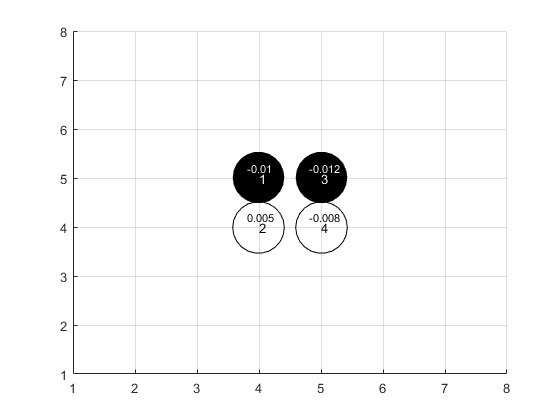
\includegraphics[width=6cm]{example/AVA1.png}
	\hspace{0.5cm}
	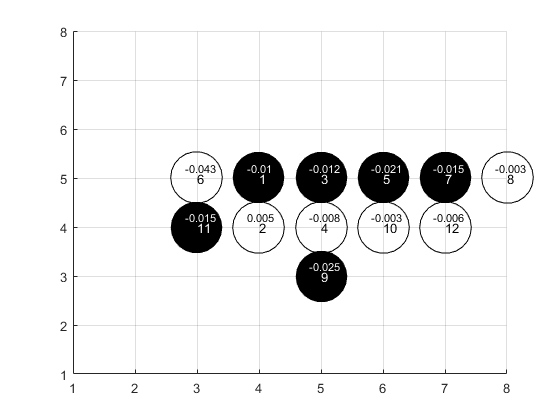
\includegraphics[width=6cm]{example/AVA2.png}
	\hspace{0.5cm}
	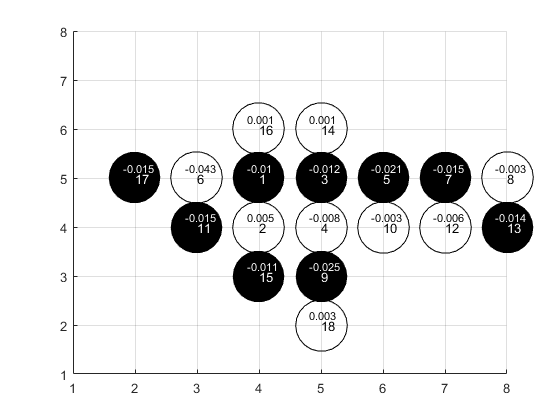
\includegraphics[width=6cm]{example/AVA3.png}
	\hspace{0.5cm}
	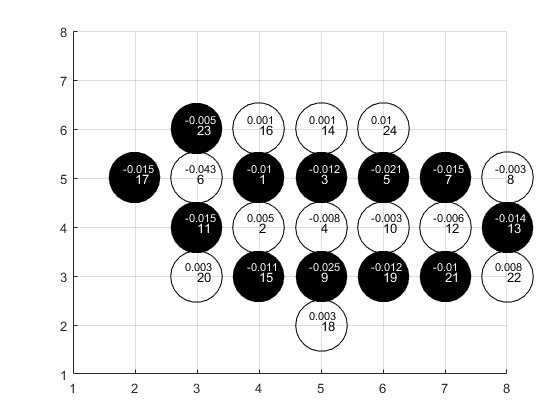
\includegraphics[width=6cm]{example/AVA4.png}
	\hspace{0.5cm}
	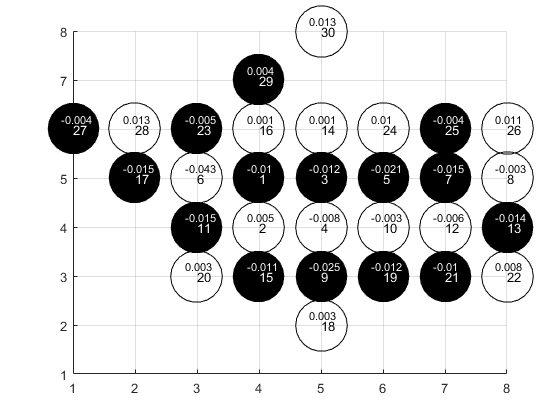
\includegraphics[width=6cm]{example/AVA5.png}
	\hspace{0.5cm}
	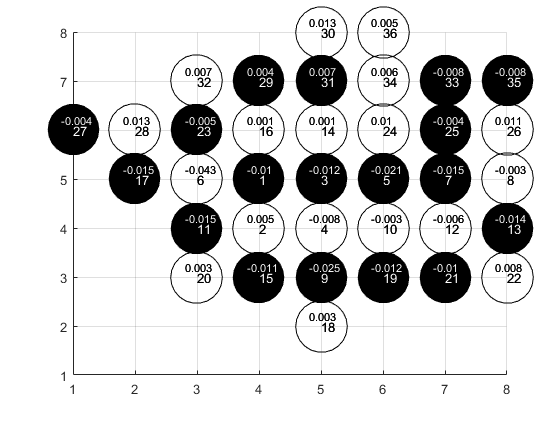
\includegraphics[width=6cm]{example/AVA6.png}
	\hspace{0.5cm}
	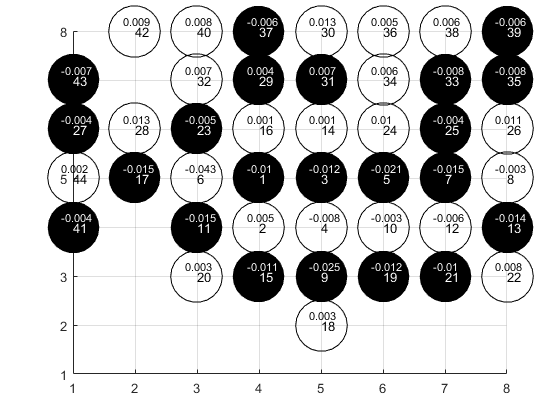
\includegraphics[width=6cm]{example/AVA7.png}
	\hspace{0.5cm}
	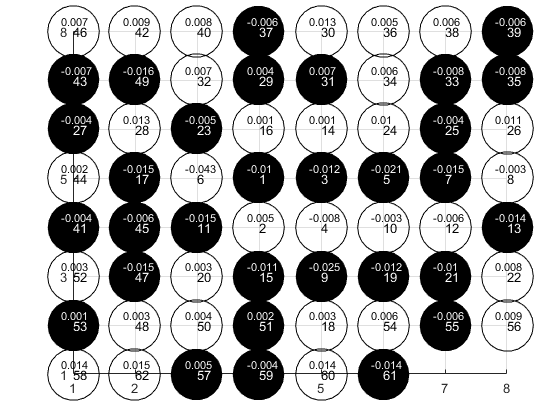
\includegraphics[width=6cm]{example/AVA8.png}
	\bicaption[这里将出现在插图索引中]
	{智能体自我博弈过程图示}
	{English caption}
	\label{fig:AIvsAI}
\end{figure}

在初始位置,神经网络对各个位置落子的概率如下:
\begin{table}[t]
	\centering
	\caption{股票数据回归结果}
\begin{tabular}{|c|c|c|c|c|c|c|c|}
	\hline 
	1.475e-4 & 1.060e-4 & 5.279e-5 & 1.107e-4 & 9.022e-5 & 4.170e-5 & 1.109e-4 & 1.193e-4 \\ 
	\hline 
	1.584e-4 & 6.658e-5 & 1.091e-3 & 5.847e-4 & 7.405e-4 & 8.547e-4 & 7.423e-5 & 8.784e-5 \\ 
	\hline 
	3.247e-5 & 7.867e-4& 4.690e-2 & 8.819e-3 & 7.429e-3&4.045e-2 & 8.091e-4 & 3.269e-5 \\ 
	\hline 
	9.957e-5& 5.741e-4 & 7.397e-3 & 0.184 & 0.198 & 0.011& 5.795e-4 & 7.367e-5 \\ 
	\hline 
	6.310e-5 &6.247e-4& 9.647e-3& 0.168 & 0.178 & 1.057e-2 & 7.635e-4 & 9.389e-5 \\ 
	\hline 
	3.174e-5 & 7.434e-4 & 4.978e-2 & 1.201e-2 & 1.064e-2 & 4.221e-2 & 6.999e-4 & 3.441e-5 \\ 
	\hline 
	1.170e-4 & 5.157e-5& 8.608e-4 & 7.298e-4 & 5.024e-4 & 9.605e-4 & 4.176e-05 & 8.261e-5\\ 
	\hline 
	1.148e-4 &7.760e-5 &  5.001e-5 & 1.053e-4 & 1.379e-4 & 2.526e-05 & 6.797e-05 & 1.110e-4 \\ 
	\hline 
\end{tabular} 
\end{table}

蒙特卡洛搜索得到的各个位置的概率:
\begin{table}[b]
	\centering
	\caption{股票数据回归结果}
\begin{tabular}{|c|c|c|c|c|c|c|c|}
		\hline 
		0& 0 & 0 & 0 & 0 & 0 &  0&  0\\ 
		\hline 
		0& 0 & 0 & 0 & 0 & 0 &  0&  0\\ 
		\hline 
		0 & 0 & 0.0125 & 0.005 & 0.0025 & 0.0125 & 0 & 0 \\ 
		\hline 
		0 & 0 & 0 & 0.1925 & 0.2425 & 0.01 & 0 & 0 \\ 
		\hline 
		0 & 0 & 0.0025 & 0.2075 & 0.265 & 0.01 & 0 & 0 \\ 
		\hline 
		0 & 0 & 0.01 & 0.005 & 0.0025 & 0.015 & 0 & 0 \\ 
		\hline 
		0 & 0 & 0 & 0 & 0 & 0 & 0 & 0 \\ 
		\hline 
		0 & 0 & 0 & 0 & 0 & 0 & 0 & 0 \\  
		\hline 
\end{tabular} 
\end{table}

可以看出,模型倾向于把初始落子位置放在中间,这也符合正常规则的五子棋的下法,第一步越靠近中间越有利。从这个角度说明了网络学习到参数的有效性。这里展示两组不同的对弈结果,下图分别是智能体自我博弈过程中的落子位置:

\begin{figure}[!htp]
	\centering
	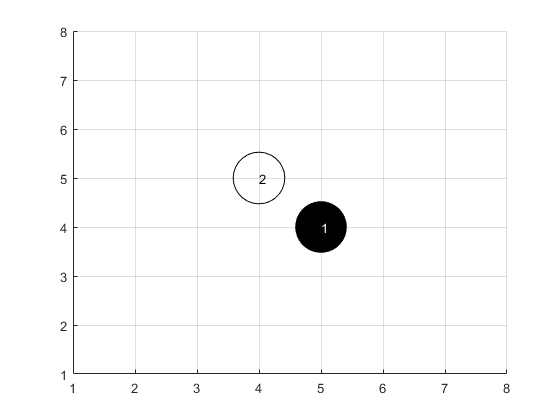
\includegraphics[width=6cm]{example/AVH1.png}
	\hspace{0.5cm}
	\bicaption[这里将出现在插图索引中]
	{智能体自我博弈过程图示}
	{English caption}
	\label{fig:AIvsAI}
\end{figure}

在下一步蒙特卡洛树得到的统计概率为:

\begin{tabular}{|c|c|c|c|c|c|c|c|}
	\hline 
	0& 0 & 0 & 0 & 0 & 0 &  0&  0\\ 
	\hline 
	0& 0 & 0 & 0 & 0 & 0 &  0&  0\\ 
	\hline 
	0 & 0 & 0.0125 & 0.005 & 0.0015 & 0.0125 & 0 & 0 \\ 
	\hline 
	0 & 0 & 0 & 0.1925 & 0.3425 & 0.02 & 0 & 0 \\ 
	\hline 
	0 & 0 & 0.0015 & 0.205 & 0.245 & 0.01 & 0 & 0 \\ 
	\hline 
	0 & 0 & 0.01 & 0.0025 & 0.005 & 0.015 & 0 & 0 \\ 
	\hline 
	0 & 0 & 0 & 0 & 0 & 0 & 0 & 0 \\ 
	\hline 
	0 & 0 & 0 & 0 & 0 & 0 & 0 & 0 \\  
	\hline 
\end{tabular} 

可以看出策略很明确,下一步的落子信息为:

\begin{figure}[!htp]
	\centering
	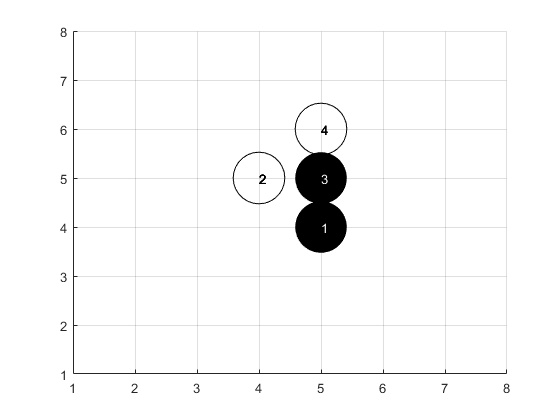
\includegraphics[width=6cm]{example/AVH2.png}
	\hspace{0.5cm}
	\bicaption[这里将出现在插图索引中]
	{智能体自我博弈过程图示}
	{English caption}
	\label{fig:human2}
\end{figure}
接下来的落子信息为:
\begin{figure}[!htp]
	\centering
	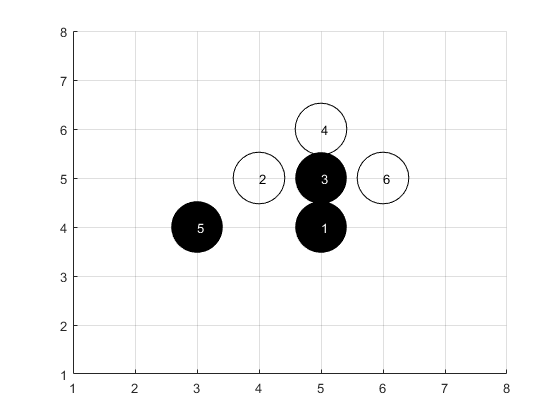
\includegraphics[width=6cm]{example/AVH3.png}
	\hspace{0.5cm}
	\bicaption[这里将出现在插图索引中]
	{智能体自我博弈过程图示}
	{English caption}
	\label{fig:human3}
\end{figure}
当模型训练好后,AI的策略是选取蒙特卡洛搜索得到的最大值贪心的进行落子。图给出了接下来几步的落子信息:
\begin{figure}[!htp]
	\centering
	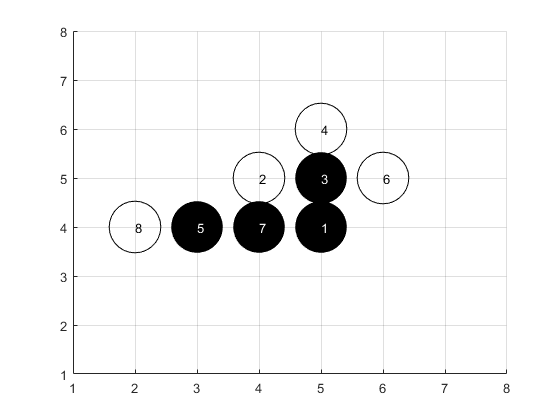
\includegraphics[width=6cm]{example/AVH4.png}
	\hspace{0.5cm}
	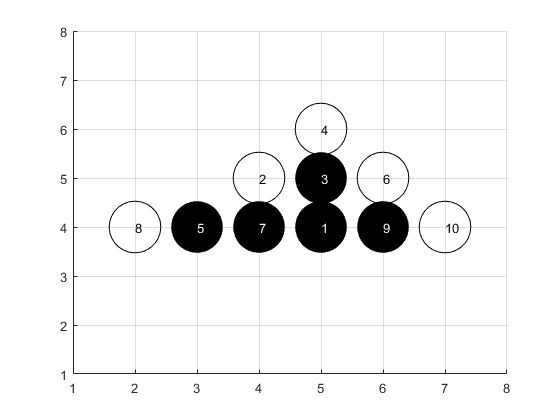
\includegraphics[width=6cm]{example/AVH5.png}
	\hspace{0.5cm}
	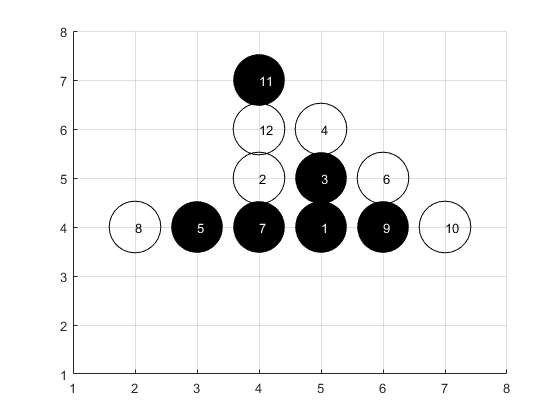
\includegraphics[width=6cm]{example/AVH6.png}
	\hspace{0.5cm}
	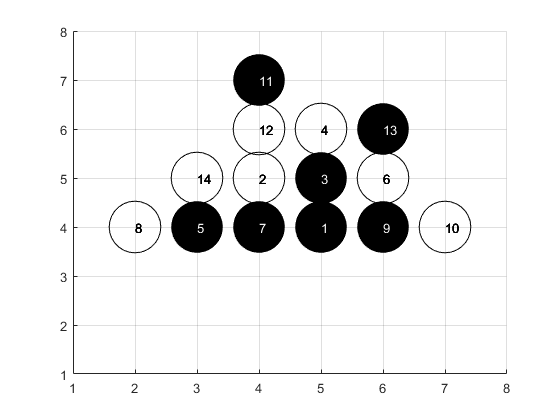
\includegraphics[width=6cm]{example/AVH7.png}
	\bicaption[这里将出现在插图索引中]
	{人机对弈过程图示}
	{English caption}
	\label{fig:AIvsHuman}
\end{figure}
%\begin{figure}[!htp]
%	\centering
%	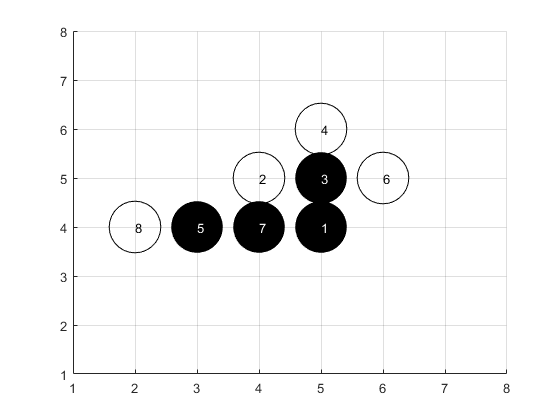
\includegraphics[width=6cm]{example/AVH4.png}
%	\hspace{0.5cm}
%		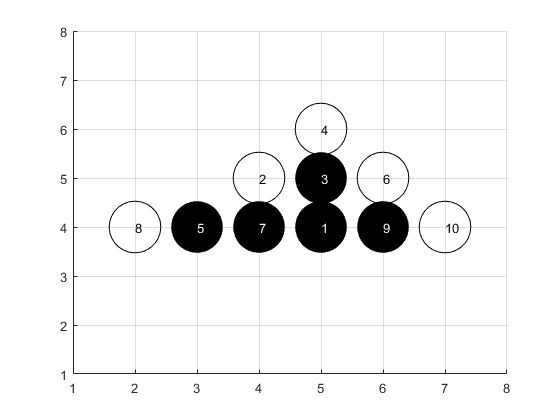
\includegraphics[width=6cm]{example/AVH5.png}
%	\hspace{0.5cm}
%		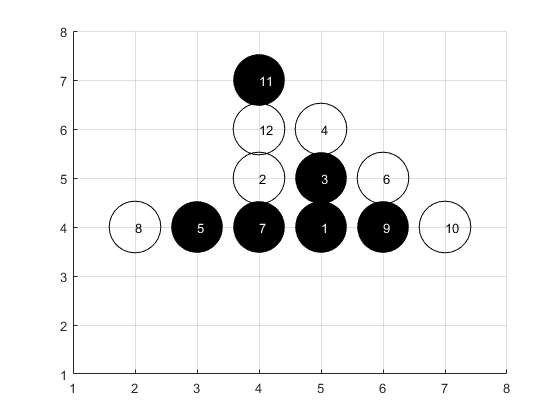
\includegraphics[width=6cm]{example/AVH6.png}
%	\hspace{0.5cm}
%		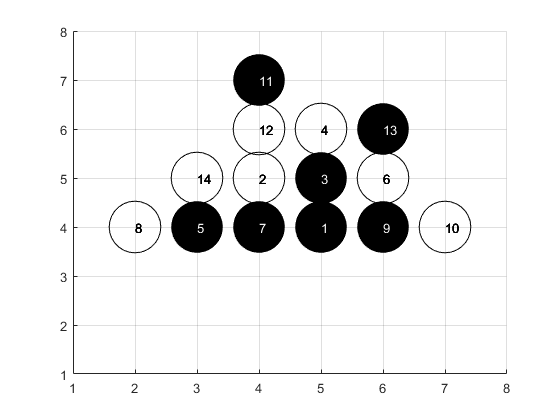
\includegraphics[width=6cm]{example/AVH7.png}
%    \hspace{0.5cm}
%	\bicaption[这里将出现在插图索引中]
%	{智能体自我博弈过程图示}
%	{English caption}
%	\label{fig:human4}
%\end{figure}
\begin{figure}[!htp]
	\centering
	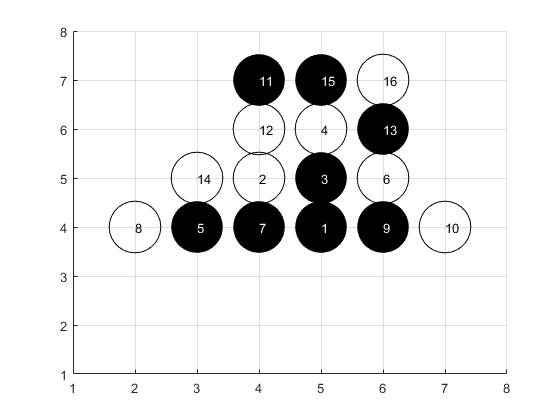
\includegraphics[width=6cm]{example/AVH8.png}
	\hspace{0.5cm}
	\bicaption[这里将出现在插图索引中]
	{智能体自我博弈过程图示}
	{English caption}
	\label{fig:human4}
\end{figure}

经过几轮对战后到达状态为图\ref{fig:human4} 第四幅图。智能体蒙特卡洛搜索得到的统计概率为:

\begin{tabular}{|c|c|c|c|c|c|c|c|}
	\hline 
	0& 0 & 0 &0  & 0 &0 0.2425 & 0 &0  \\ 
	\hline 
	0 & 0 & 0 & 0 & 0 & 0 & 0.615 & 0 \\ 
	\hline 
	0 & 0 & 0 & 0 & 0 & 0 & 0 & 0 \\ 
	\hline 
	0 & 0 & 0 & 0 & 0& 0 & 0 & 0 \\ 
	\hline 
	0 & 0 & 0.135 & 0 & 0.0025 & 0 & 0 & 0.0025 \\ 
	\hline 
	0 & 0 & 0 & 0 & 0 & 0 & 0 & 0 \\ 
	\hline 
	0 & 0 & 0 & 0 & 0 & 0 & 0 & 0 \\ 
	\hline 
	0 & 0 & 0 & 0 & 0 & 0 & 0 & 0 \\ 
	\hline 
\end{tabular}

选择概率最大的进行动作,得到如下状态:

\begin{figure}[!htp]
	\centering
	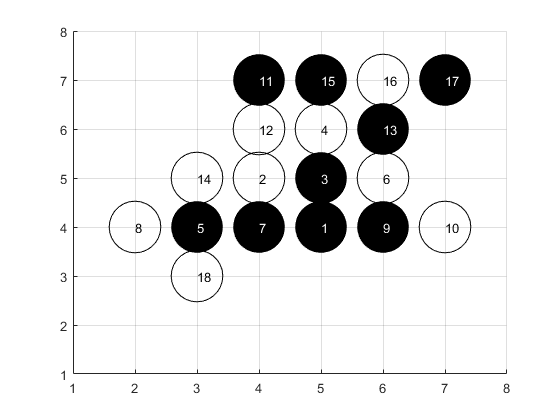
\includegraphics[width=6cm]{example/AVH9.png}
	\hspace{0.5cm}
	\bicaption[这里将出现在插图索引中]
	{智能体自我博弈过程图示}
	{English caption}
	\label{fig:human5}
\end{figure}

这时策略神经网络输出概率值信息为:

\begin{tabular}{|c|c|c|c|c|c|c|c|}
	\hline 
	4.364e-3 & 1.047e-3 & 7.525e-3 & 2.883e-3 & 6.946e-4 & 5.545e-3 & 0.057 & 0.309 \\ 
	\hline 
	3.495e-3 & 1.008e-2 & 9.739e-3 & 7.828e-05 & 1.271e-3 & 3.174e-05 & 7.719e-4 & 7.758e-4 \\ 
	\hline 
	5.235e-4 & 7.740e-3 & 6.412e-4 & 5.572e-05 & 1.263e-06 & 1.740e-4 & 3.681e-3 & 6.366e-4 \\ 
	\hline 
	7.379e-2 & 1.574e-2 & 6.703e-07 & 6.327e-06 & 3.206e-05 & 1.603e-05 & 5.863e-2 & 9.232e-3 \\ 
	\hline 
	2.077e-4 & 1.737e-05 & 1.134e-4 & 2.158e-05 & 2.920e-06 & 1.697e-4 & 5.049e-4 & 2.913e-2 \\ 
	\hline 
	9.056e-2 & 1.897e-2 & 3.469e-06 & 2.165e-3 & 2.638e-3 & 1.505e-3 & 1.165e-2 & 0.128 \\ 
	\hline 
	8.939e-4 & 2.178e-4 & 4.440e-4 & 8.316e-2 & 1.967e-3 & 8.452e-4 & 5.612e-4 & 4.942e-4 \\ 
	\hline 
	9.371e-4 & 6.839e-4 & 4.050e-3 & 3.668e-4 & 2.882e-2 & 3.848e-4 & 6.134e-4 &5.001e-4 \\ 
	\hline 
\end{tabular} 

蒙特卡洛树统计得到的概率信息为:

\begin{tabular}{|c|c|c|c|c|c|c|c|}
	\hline 
	0& 0 & 0 &0  & 0 &0  & 0.03 &0.625  \\ 
	\hline 
	0 & 0 & 0.0225 & 0 & 0 & 0 & 0 & 0 \\ 
	\hline 
	0 & 0 & 0 & 0 & 0 & 0 & 0.1 & 0 \\ 
	\hline 
	0 & 0 & 0 & 0 &0 & 0 & 0 & 0 \\ 
	\hline 
	0 & 0 &0& 0 & 0 & 0 & 0 & 0.07\\ 
	\hline 
	0 & 0 & 0 & 0 & 0.0575 & 0 & 0 & 0 \\ 
	\hline 
	0 & 0 & 0 & 0 & 0 & 0 & 0 & 0 \\ 
	\hline 
	0 & 0 & 0 & 0.0725 & 0 & 0 & 0 & 0 \\ 
	\hline 
\end{tabular}

这时观察当前状态对于黑方叶子节点预测奖励为0.97883,根据贪心策略选择概率最大的动作执行,得到下面的状态信息:

\begin{figure}[!htp]
	\centering
	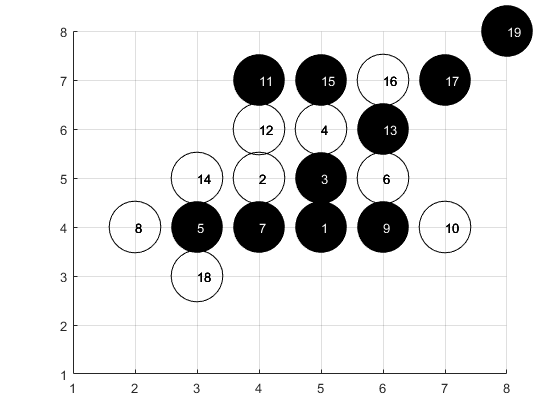
\includegraphics[width=6cm]{example/AVH10.png}
	\hspace{0.5cm}
	\bicaption[这里将出现在插图索引中]
	{智能体自我博弈过程图示}
	{English caption}
	\label{fig:human6}
\end{figure}

最后黑方获胜,通过实验可知距离奖励越近策略越明确,在本实验中,观察策略网络输出的交叉熵可以看出智能体在训练过程中随着迭代的进行策略越接近于明确,损失函数不断下降。在人机博弈时,神经网络基本能准确输出各个位置获胜的概率,和蒙特卡洛树统计得到的概率基本一致。在游戏结束时,奖励越来越明确,智能体也能准确感知当前的状态信息并作出决策。在自我博弈过程中,连个智能体相互对抗直到和棋,说明训练出的智能体基本棋力相当,也证明了用自我博弈方式产生数据的有效性。由于棋盘过小,硬件资源有限,这里只给出了8*8的情况,又由于强化学习训练比较困难,稳定性不高,在本章只介绍了对于对称类棋盘博弈的相关实验,对于其他应用场景的拓展还有待开发。
\section{本章小结}
本章主要针对对称类双人棋盘博弈模型进行探索和研究。在文章的第一部分介绍了博弈模型的概念和类别,第二部分介绍了AlphaGo和AlphaZero的基本原理,其主要的组成部分有蒙特卡洛搜索树,深度学习网络和强化学习基本原理。首先利用蒙特卡洛搜索树建立两个智能体相互博弈的模型,在树的叶子节点选择过程中用到了强化学习最大化奖励函数的原理,在叶子节点扩展中需要结合深度学习网络进行动作和值函数的估计,然后把多次模拟的数据进行统计,作为深度学习网络的拟合标签,以更新后的深度学习网络为基础进行下一次树的建立。最后策略网络就是模型得到的最终结果。AlphaGo利用了人类监督数据进行网络的初始化处理以及搜索树的快速走子,AlphaZero则从无到有完全利用自我博弈数据进行深度学习网络的拟合。针对于强化学习探索和利用的平衡问题以及在深度学习网络更新中学习率难以选择的问题,在本章的第三部分提出了两点改进:受多臂老虎机模型的启发,这里用温度系数控制动作选择部分对探索和利用的平衡,避免因探索权重大带来的计算复杂度高和利用权重大带来模型陷入局部最优解的问题,为了进一步避免动作过于单一,在概率分布上加入随机噪声。用相对熵衡量策略网络输出参数的相对变化范围,根据网络参数的变化自适应调整学习率,在网络训练前期加快步长,在接近最优解时减小步长,既能提高训练效率又能避免局部最优。在文章的第四部分针对改进的方案结合五子棋模型原型讨论了在不同温度系数和不同学习率参数下网络损失函数和交叉熵的变化曲线,根据输出曲线合理选择网络的参数。在第五部分针对改进算法设计了五子棋实验,展示了人机对战结果和智能体之间自博弈结果。针对人机博弈过程详细展示了蒙特卡洛搜索树搜索结果和神经网络输出概率值,在结果上验证了改进算法的可行性。